\chapter{Eficiencia del trigger de fotones}
% \addcontentsline{toc}{chapter}{Eficiencia del trigger de fotones}
\chaptermark{Eficiencia del trigger de fotones}


En la Sección \ref{sec:trigger} se detalló el funcionamiento del sistema de trigger y su importancia para los distintos análisis que se realizan dentro de la colaboración. La medida precisa de la eficiencia de los triggers es empleada para tener conocimiento del rendimiento de los mismos y poder entonces determina la aceptancia de los análisis físicos de interés que involucran cada uno de los triggers utilizados. 
En este Capítulo se discute en particular la medida de la eficiencia de los triggers de fotones, que son de especial importancia para esta tesis, y a su vez se detalla el cálculo de los factores de escala asociados a dichas eficiencia . El método empleado se basa una muestra de datos con fotones de alta pureza seleccionados a partir de eventos con bosones $Z$ que decaen radiativamente. Este método se utiliza para la medida de la eficiencia de triggers con fotones de bajo \ET, debido a la baja estadística de la muestra cuando los fotones tienen $\ET>60\,\gev$. Complementariamente, para triggers con fotones de mayor \ET, se utiliza otro método denominado \textit{Bootstrap}, que tiene una mayor estadística en ese rango a costa de una menor pureza, el cual no es descripto en esta Tesis.

La medida de la eficiencia de los triggers de fotones y el cálculo de su factores de escala fueron hechos bajo el marco de la \textit{ATLAS Qualification}, un trabajo de un año de servicio, obligatorio para nuevos ingresantes, y requisito para ser miembro de la colaboración. Tales resultados son empleados por todos los análisis que usen los triggers de fotones primarios para la selección de eventos.

% \solved{Justificar o motivar de una mejor forma el por qué explicamos el método del Zrad si los triggers que usamos en el análisis son medidos con Bootstrap} Done!


\section{Reconstrucción de fotones en el trigger}

La reconstrucción de fotones \cite{TRIG-2018-05} (y de forma similar la de electrones) en el trigger comienza en el L1 con la construcción de regiones de interés (RoIs) utilizando sólo la información del calorímetro. A partir de esas RoIs el HLT ejecuta algoritmos de reconstrucción rápida que utilizan adicionalmente información del detector interno dentro de la RoI, permitiendo una selección e identificación inicial de fotones junto con un temprano rechazo de fondo. En el caso de que el candidato cumpla los requisitos de selección rápidos se ejecuta a continuación los algoritmos de precisión, que utilizan información adicional en regiones del detector fuera de la RoI. Estos algoritmos son similares a los utilizados en la reconstrucción offline con la diferencia de que no reconstruyen superclusters de fotones. Utilizando sólo la información del calorímetro es suficiente para tener una alta eficiencia por lo que los mismos son reconstruidos bajo la hipótesis de que no son convertidos, no se reconstruyen trazas ni se aplican criterios de ambigüedad con los electrones, reduciendo notablemente el consumo de CPU. 
% \solved{tampoco hace ambiguity con electrons, los electrones pueden pasar el trigger de fotones!!!} lo puse
A continuación se detallan los mecanismos realizados en ambas etapas del trigger.

\subsubsection{Reconstrucción de fotones en el L1}

Los triggers del L1 utiliza la información del calorímetro en la región central ($|\eta|<2.5$) para construir las RoIs, que consisten en torres (\textit{trigger towers}) de $4\times4$ celdas del calorímetro de $0.1\times0.1$ en $\eta$ y $\phi$. Un algoritmo (\textit{sliding-window} \cite{Lampl:1099735}) busca los conjuntos de celdas de $2\times2$ cuya suma de energía transversa de uno de los cuatro posibles pares de celdas vecinas más cercanas ($1\times2$ o $2\times1$) supere el umbral de energía que define al trigger. La Figura \ref{fig:l1_reco} muestra un esquema de una torre de trigger que emplea dicho algoritmo, mientras que en la Figura \ref{fig:ecal} se detalla la región del ECAL que representa una torre del trigger.

\begin{figure}
  \centering
  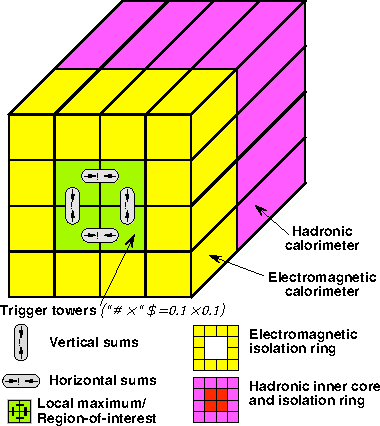
\includegraphics[width=0.35\textwidth]{images/trigger/l1_reco.pdf}
  \caption{Esquema de torre de trigger empleada por los algoritmos del L1 \cite{TRIG-2016-01}.}
  \label{fig:l1_reco}
\end{figure}


Este umbral puede depender de $\eta$ con una granularidad de $0.1$, en general variando entre \magn{-2}{GeV} y \magn{3}{GeV} con respecto al umbral nominal, y en ese caso se agrega una letra `V' al final del nombre del trigger. A su vez se puede aplicar un rechazo de actividad hadrónica, donde se descarta al candidato si la suma de energía transversa de las celdas en el calorímetro hadrónico de la ventana de $2\times2$ es mayor a \magn{1}{GeV} y supera $\ET/23\,\gev-0.2\,\gev$. En ese caso se agrega una `H' al final del nombre del trigger. Finalmente se puede incluir requisitos de aislamiento que rechazan a los candidatos si la suma de la energía transversa en las 12 celdas alrededor de la ventana de $2\times2$ es mayor a \magn{2}{GeV} y supera $\ET/8\,\gev-1.8\,\gev$, agregando una `I' al nombre del trigger. Por ejemplo, el trigger \texttt{L1\_EM20VHI} tiene un umbral de \magn{20}{GeV} variable en $\eta$ y utiliza el rechazo hadrónico y la selección de aislamiento. Tanto el rechazo hadrónico como la selección de aislamiento se aplican solamente a triggers con umbral mayor a \magn{50}{GeV}.

\subsubsection{Reconstrucción de fotones en el HLT}

La reconstrucción en el HLT comienza aplicando algoritmos de reconstrucción rápida para reconstruir clusters con las celdas de las RoIs obtenidas en el L1. Para acelerar el proceso estos algoritmos solo utilizan la segunda capa del calorímetro electromagnético para encontrar la celda con mayor energía transversa de la RoI (semilla). La posición del cluster se obtiene calculando el promedio de las posiciones pesadas por la energía
% energy–weighted average cell positions  
 % \commentred{entender y traducir} Done!
dentro de una ventana de $3\times7$ ($\Delta\eta\times\Delta\phi = 0.075\times0.175$) centrada en la celda semilla. Para calcular la energía acumulada 
en todas las capas del calorímetro
se utiliza una ventana de $3\times7$ ($\Delta\eta\times\Delta\phi = 0.075\times0.175$) en la región barrel y una ventana de $5\times5$ ($\Delta\eta\times\Delta\phi = 0.125\times0.125$) en el endcap. Adicionalmente se realizan correcciones basadas en los algoritmos de reconstrucción que mejoran la resolución de la posición y energía del cluster. En esta etapa se realizan selecciones solamente basadas en la energía transversa del cluster y en los parámetros $R_{\text{had}}$, $R_{\eta}$ y $E_{\text{ratio}}$.


Si el candidato pasa la selección anterior se utiliza una región levemente mayor a la RoI para ejecutar los algoritmos de precisión. Estos algoritmos son los mismos empleados en la reconstrucción offline \cite{Lampl:1099735} para construir el clusters y técnicas multivariable \cite{PERF-2017-03} para hacer correcciones en su energía. La identificación online de fotones utiliza las mismas variables discriminatorias que en la reconstrucción offline, definiendo tres WPs: \texttt{Loose}, \texttt{Medium} (empleado solamente en el HLT), y \texttt{Tight}.
Adicionalmente es posible incluir requisitos de aislamiento calorimétrico utilizando topo-clusters, de forma similar a la reconstrucción offline. Para ello se reconstruye la totalidad de los topo-clusters presentes en el evento para calcular la densidad de energía del evento en el HLT, necesaria para sustraer el ruido de la señal en el cono de aislamiento. El cono se construye con un radio de  $\Delta R < 0.2\:(0.4)$ alrededor del candidato para el punto de trabajo de aislamiento \texttt{Very-Loose} (\texttt{Tight}), denotado en el nombre del trigger como \texttt{icalovloose} (\texttt{icalotight}). Un fotón en el HLT se considera aislado si la fracción entre la energía transversa del topo-cluster y la del candidato es menor a
% \commentyellow{if the ratio of the transverse energy in the topo-clusters to the transverse energy of the photon candidate is less than: no me queda claro donde entra el cono acá...} 
10\% (3\% con un corrimiento de energía de \magn{2.45}{GeV} similar al de la Tabla \ref{tab:IDWPs}). La reconstrucción de los topo-clusters del evento se realiza una sola vez en el evento y es utilizado por todos los triggers, inclusive aquellos que no utilizan fotones. 

% No iria esta iamgen...
% La Figura \ref{fig:hlt_alg} muestra un esquema del algoritmo empleado para la reconstrucción de fotones en le HTL.

% \begin{figure}
%   \centering
%   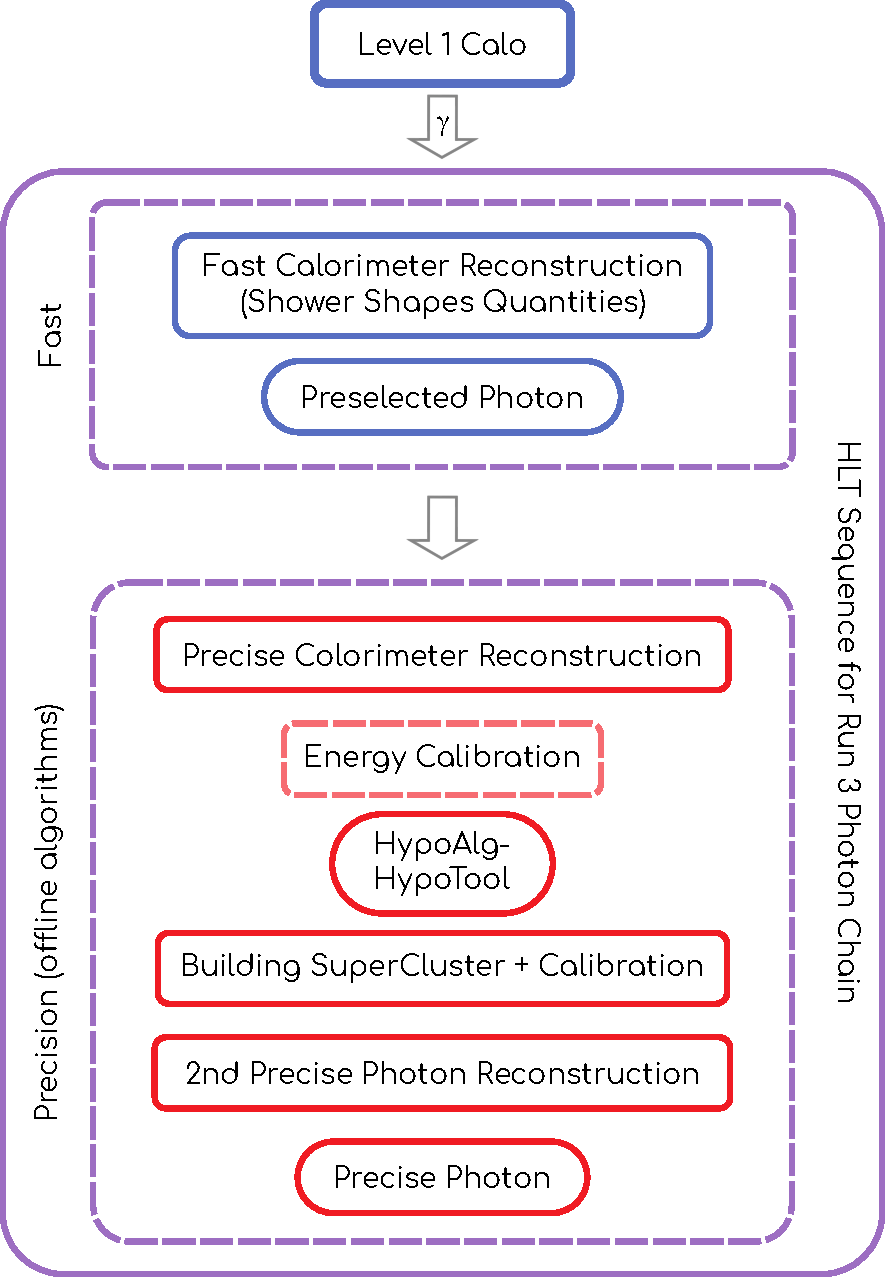
\includegraphics[width=0.45\textwidth]{images/trigger/hlt_alg.pdf}
%   \caption{Esquema del algoritmo empleado para la reconstrucción de fotones en el HLT. }
%   \label{fig:hlt_alg}
% \end{figure}


\section{Nomenclatura y trigger primarios de fotones}


% / Representado en imagen al final
% {\footnotesize \texttt{`Nivel de trigger'\_`Multiplicidad del objeto'`Tipo de objeto'`Umbral de \ET'\_`Requisitos adicionales'}}


A continuación se describe convención de nombres de triggers utilizada en el detector ATLAS.
El nivel del trigger puede ser tanto L1 como HLT. La multiplicidad representa la cantidad de objetos que pretende seleccionar el trigger con esos mismo requisitos. Los posibles tipos de objetos para los triggers de fotones pueden ser `EM' en el caso de triggers del L1 y `g' para el HLT. En el caso de triggers del L1 es posible que incluyan los requisitos `I', `H' o `V' descriptas anteriormente. Los triggers compuestos por la disyunción de otros dos trigger, incluyen ambas componentes en el nombre sucesivamente. Finalmente en los requisitos adicionales se incluye la identificación, y en caso de haber requisito de aislamiento se agrega a continuación. Opcionalmente para los HLT triggers se puede explicitar el trigger del L1 que se utilizó como semilla. En la Figura \ref{fig:trigger_name} se muestra un ejemplo de nomenclatura para el trigger \texttt{HLT\_2g20\_tight\_icalovloose\_L12EM15VHI}, el cual representa un trigger del HLT que selecciona eventos con al menos dos fotones con $\ET>20\,\gev$, ambos que pasen los requisitos de identificación \texttt{Tight} y de aislamiento \texttt{icalovloose}, y adicionalmente se especifica el seed L1 trigger que requiere de dos L1 EM clusters con un umbral dependiente en $\eta$ y centrado en \magn{15}{GeV}, con los requisitos de aislamiento y rechazo hadrónico.

\begin{figure}
  \centering
  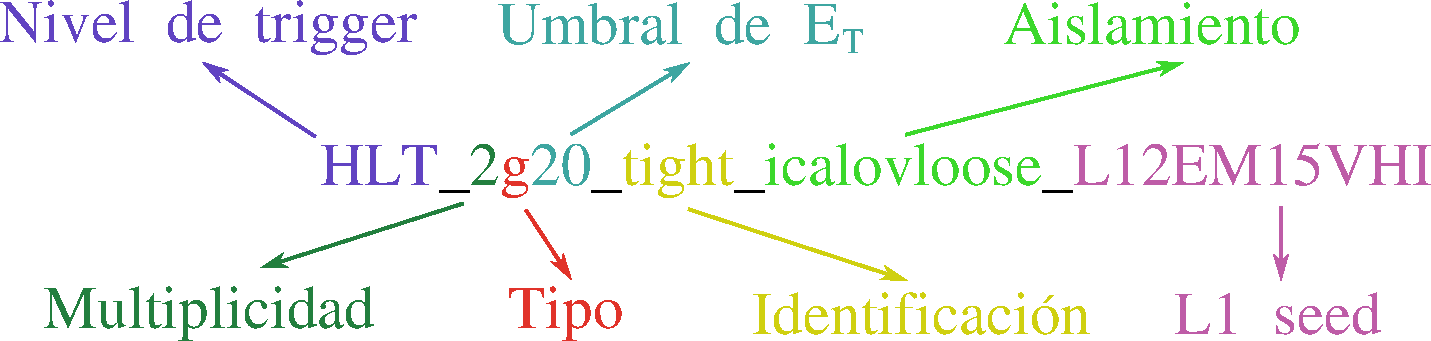
\includegraphics[width=0.8\textwidth]{images/trigger/trigger_name.pdf}
  \caption{Convención para la nomenclatura de los triggers en ATLAS.}
  \label{fig:trigger_name}
\end{figure}

Los principales triggers de fotones se detallan en la Tabla \ref{tab:prim_ph_trig}. El trigger primario de un fotón con menor umbral y sin prescale 
% \solved{Lo voy a definir en el capitulo del LHC/Trigger} Done!
está diseñado para búsquedas de física nueva más allá del SM con fotones de alto \ET, mientras que el de dos fotones se utiliza principalmente para seleccionar eventos con bosones de Higgs decayendo a fotones. Los triggers de dos fotones con umbrales bajos e identificación \texttt{Tight} son empleados para estudios más allá del SM con resonancias de baja masa ($\sim60\,\gev$).



\begin{table} 
\caption{Triggers principales de fotones utilizados a lo largo de cada año durante el Run 2.}
	\centering
\resizebox{\linewidth}{!}{
	\begin{tabular}{ l | c | c | c }

	 \hline
	  \hline
		Tipo de trigger & 2015 & 2016 & 2017-2018 \\

		\hline
		\hline

		L1 simple & \texttt{L1\_EM20VH} & \multicolumn{2}{c}{\texttt{L1\_EM22VHI}} \\

		\hline

		L1 doble & \texttt{L1\_2EM10VH} & \texttt{L1\_2EM15VH} & \texttt{L1\_2EM15VHI} \\

		\hline

		Primario simple & \texttt{HLT\_g120\_loose} & \multicolumn{2}{c}{\texttt{HLT\_g140\_loose}} \\

		\hline
		
		Primario doble & \multicolumn{2}{c|}{\texttt{HLT\_g35\_loose\_g25\_loose}} & \texttt{HLT\_g35\_medium\_g25\_medium} \\

		\hline
		
		\texttt{Loose} doble & \multicolumn{2}{c|}{-} & \texttt{HLT\_2g50\_loose} \\

		\hline
		
		\texttt{Tight} doble & \texttt{HLT\_2g20\_tight} & \texttt{HLT\_2g22\_tight} & \texttt{HLT\_2g20\_tight\_icalovloose} \\

		\hline
		\hline

	\end{tabular}


}
	\label{tab:prim_ph_trig}
\end{table}




\section{Método del bosón $Z$ decayendo radiativamente}

Debido al amplio conocimiento adquirido en las últimas décadas sobre las propiedades del bosón $Z$, el mismo es empleado en la actualidad para realizar medidas de calibración y eficiencia. El decaimiento radiativo del bosón $Z$ ocurre cuando uno de los productos del decaimiento leptónico irradia un fotón ($Z\to l^{+}l^{-}\gamma,\:l=e,\mu$). Este decaimiento en particular se utiliza cuando se desea obtener una muestra de fotones con una elevada pureza, debido a que al reconstruir la masa invariante de los tres objetos y requerir que sea compatible con la del bosón $Z$, la posibilidad de que el fotón haya sido erróneamente reconstruido es muy baja. Teniendo en cuenta la alta pureza de fotones de la muestra esta técnica no requiere de métodos de sustracción de fondo. La desventaja de este método es la baja estadística de eventos con estas características cuando el \pt del fotón es alto, por lo que es utilizado para medir eficiencias de triggers con umbrales menores a \magn{60}{GeV}.

En el contexto de este trabajo, la eficiencia de un determinado trigger se define como la fracción de eventos que pasaron el mismo con respecto al total de eventos presentes en la muestra:

\begin{equation}
	\epsilon = \frac{N_\text{trig}}{N_\text{total}}
	\label{eq:trig_eff}
\end{equation}

La eficiencia se calcula en función de distintas variables como por ejemplo \ET y $\eta$ del fotón reconstruido offline, o el $\langle\mu\rangle$ del evento. En el caso de una eficiencia teórica en función del \ET la forma de la misma debería ser una función escalón de Heaviside centrada en el valor de corte de \ET del trigger. El sistema de trigger toma una decisión basada en la reconstrucción de objetos online o tiempo real, sin embargo para los análisis físicos los objetos de interés son los reconstruidos offline de mayor precisión. Es por esto que las eficiencias se evalúan con respecto a estos últimos objetos, observando entonces un desvanecimiento de la curva escalón en el valor de selección online, en la llamada región de encendido (\textit{turn-on}) del trigger en estudio. 
Los triggers y algoritmos de reconstrucción e identificación están diseñados para impedir una dependencia de la eficiencia en $\eta$ o $\langle\mu\rangle$, por lo que al expresarla en función de estas variables se espera una curva plana muy cercana a 1. En el caso de triggers compuestos, se calcula la eficiencia de cada componente y la eficiencia total resulta como el producto de ambas.

% no se que quise poner en la primer oracion , pero mande todo mas abajo y de forma correcta
% La medida de la eficiencia de cada trigger utiliza los datos tomados en el año correspondiente al mismo, listados en la Tabla \ref{tab:prim_ph_trig}. En el caso de que el trigger o una de sus componentes se haya configurado con un prescale, el mismo se emplea en modo rerun para la medida de la eficiencia. 


A los eventos se les solicita tener al menos dos leptones de carga opuesta y un fotón, todos con $\pt>10\,\gev$. El fotón debe estar dentro de la región $|\eta| < 2.37$ y pasar el WP de identificación \texttt{Tight}. Las eficiencias se calculan para los distintos WPs de aislamiento del fotón utilizado, en este caso para \texttt{FixedCutTightCaloOnly} y \texttt{FixedCutLoose}. Los leptones deben estar dentro de la región $|\eta| < 2.47$, pasar el WP de identificación \texttt{Medium}, el de aislamiento \texttt{FixedCutLoose} y su traza asociada tener $|z_0| < 10$ mm y $\sigma(d_0) < 10$. A su vez el evento es rechazado si el $\Delta R$ entre el fotón y alguno de los leptones es menor a 0.2. Finalmente se realiza una selección en la masa invariante de los leptones ($m_{ll}$) y la de los 3 objetos ($m_{ll\gamma}$). En la Figura \ref{mllgmll} se muestra el gráfico de $m_{ll}$ en función de $m_{ll\gamma}$. En la misma se puede observar que la mayoría de los eventos se encuentra en la región $m_{ll}\sim91\,\gev$ y $m_{ll\gamma}>\sim96\,\gev$, estos representan eventos en los cuales un bosón $Z$ decayó a un par de leptones, y que adicionalmente en el evento se encontraba un fotón proveniente de otro proceso. En cambio en la región $86\,\gev<m_{ll\gamma}<96\,\gev$ y $40\,\gev<m_{ll}<83\,\gev$ la masa invariante de los pares de leptones no alcanza la del bosón $Z$, pero al combinarlos con el fotón sí lo hace. Al aplicar este último corte se garantiza que un leptón necesariamente haya irradiado y que el fotón provenga del decaimiento del bosón $Z$ y no de otro proceso. En el caso de tener en el evento más de un fotón o más de dos leptones que cumplan los requisitos, se seleccionó el trío cuya masa invariante sea la más cercana a la del bosón $Z$.

\begin{figure}
  \centering
  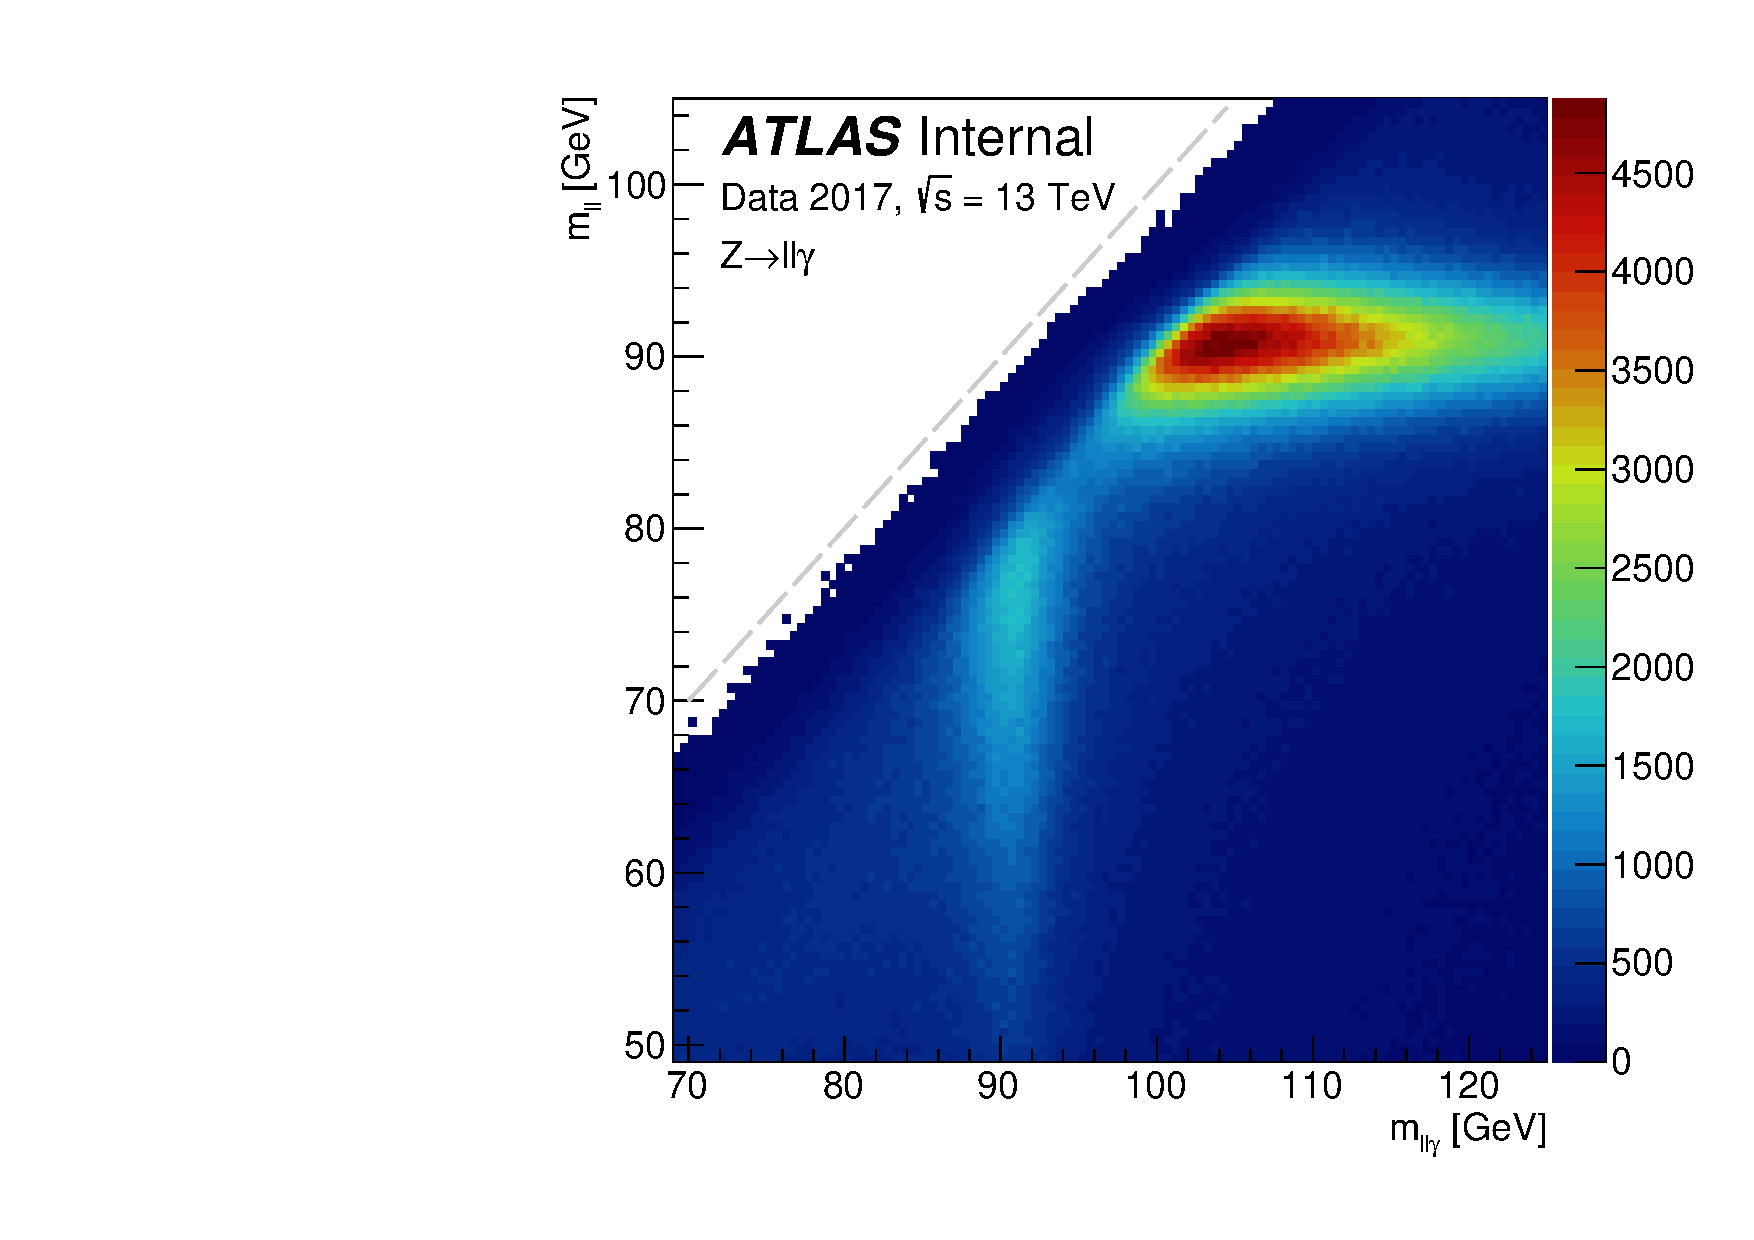
\includegraphics[width=0.6\textwidth]{images/trigger/h_mllg_mll.pdf}
	\caption{Masa invariante de dos leptones en función de la masa invariante de ambos leptones junto con un fotón. Las regiones con mayor concentración de eventos representan el decaimiento de un bosón $Z$ a leptones o de forma radiativa.}
  \label{mllgmll}
\end{figure}

La muestra de datos se obtiene a partir de eventos que pasaron los triggers primarios de electrones o muones, utilizando la derivación \texttt{EGAM3} (\texttt{EGAM4}) que preselecciona eventos con dos electrones (muones) y un fotón, con requisitos orientados a este tipo de decaimiento, descriptos en la Sección \ref{sec:lhc_samples}. El uso de triggers de leptones se debe aque si se utilizaran triggers de fotones se podría estar introduciendo un sesgo en las eficiencias.

Finalmente las eficiencias se obtienen contando el número de eventos que pasa esta selección, y que representa el denominador en la Ecuación \ref{eq:trig_eff}. Para el numerador se cuenta cuántos de esos eventos, el fotón presente en el mismo pasó la selección del trigger a evaluar. Las eficiencias fueron calculadas para los triggers listados en la Tabla \ref{tab:trigg_eff}, empleando los datos correspondientes a su año. Las mismas son calculadas en función de \ET para fotones fuera de la región crack, y de $\eta$ y $\langle\mu\rangle$ para fotones con \ET mayor a \magn{5}{GeV} del umbral del trigger. En el caso de que el trigger o una de sus componentes se haya configurado con un prescale, el mismo se emplea en modo rerun para la medida de su eficiencia. En las Figuras \ref{fig:photon_trig_eff_2015}, \ref{fig:photon_trig_eff_2016}, \ref{fig:photon_trig_eff_2017} y \ref{fig:photon_trig_eff_2018} se pueden observar algunos de dichos resultados en función de distintas variables. En general todas son cercanas a la unidad y constantes, salvo para $\langle\mu\rangle$ que se observa una pequeña dependencia algo esperable dado el incremento de colisiones por cruce de haces. Esto se ve en mayor medida en los triggers \texttt{HLT\_g20\_tight\_icalovloose\_L1EM15VHI} y \texttt{HLT\_g22\_tight\_L1EM15VHI} debido a que 
el aislamiento en el L1 no contemplaba ninguna corrección por pile-up.
% \solved{No recuerdo bien a qué se debía esta disminución en la eficiencia, algo del seed del L1?}. Done!
En la Figura \ref{fig:bs_vs_zrad} se muestra una comparación de las eficiencias calculadas con el método Bootstrap \cite{tesis_joaco} y el método del bosón $Z$ radiativo para un mismo trigger, en la que se puede observar una pequeña mejora en la eficiencia utilizando este último método, lo que motiva a su uso para triggers de bajo \ET.

\begin{table}
	\centering
	\caption{Triggers de fotones para los cuales se calcularon sus eficiencias y su respectivo año.}
	\begin{tabular}{ l | l | l | l | l }

		\hline
		\hline

		Trigger & 2015 & 2016 & 2017 & 2018 \\

		\hline
		\hline

		\texttt{HLT\_g15\_loose} & \cmark & \cmark &  &  \\
		\texttt{HLT\_g15\_loose\_L1EM3} &  &  & \cmark & \cmark \\
		\texttt{HLT\_g20\_loose} & \cmark & \cmark &  &  \\
		\texttt{HLT\_g20\_tight} & \cmark & \cmark &  &  \\
		\texttt{HLT\_g20\_tight\_icalovloose\_L1EM15VHI} &  &  & \cmark & \cmark \\
		\texttt{HLT\_g22\_tight} &  & \cmark &  &  \\
		\texttt{HLT\_g22\_tight\_L1EM15VHI} &  &  & \cmark & \cmark \\
		\texttt{HLT\_g25\_loose} & \cmark & \cmark & \cmark & \cmark \\
		\texttt{HLT\_g25\_loose\_L1EM15} & \cmark &  &  &  \\
		\texttt{HLT\_g25\_medium\_L1EM20VH} &  &  & \cmark & \cmark \\
		\texttt{HLT\_g35\_loose} & \cmark & \cmark &  &  \\
		\texttt{HLT\_g35\_medium\_L1EM20VH} &  &  & \cmark & \cmark \\
		\texttt{HLT\_g35\_loose\_L1EM15} & \cmark &  &  &  \\
		\texttt{HLT\_g50\_loose\_L1EM20VH} &  &  & \cmark & \cmark \\

		\hline
		\hline

	\end{tabular}
	\label{tab:trigg_eff}
\end{table}





\begin{figure}
  \centering
  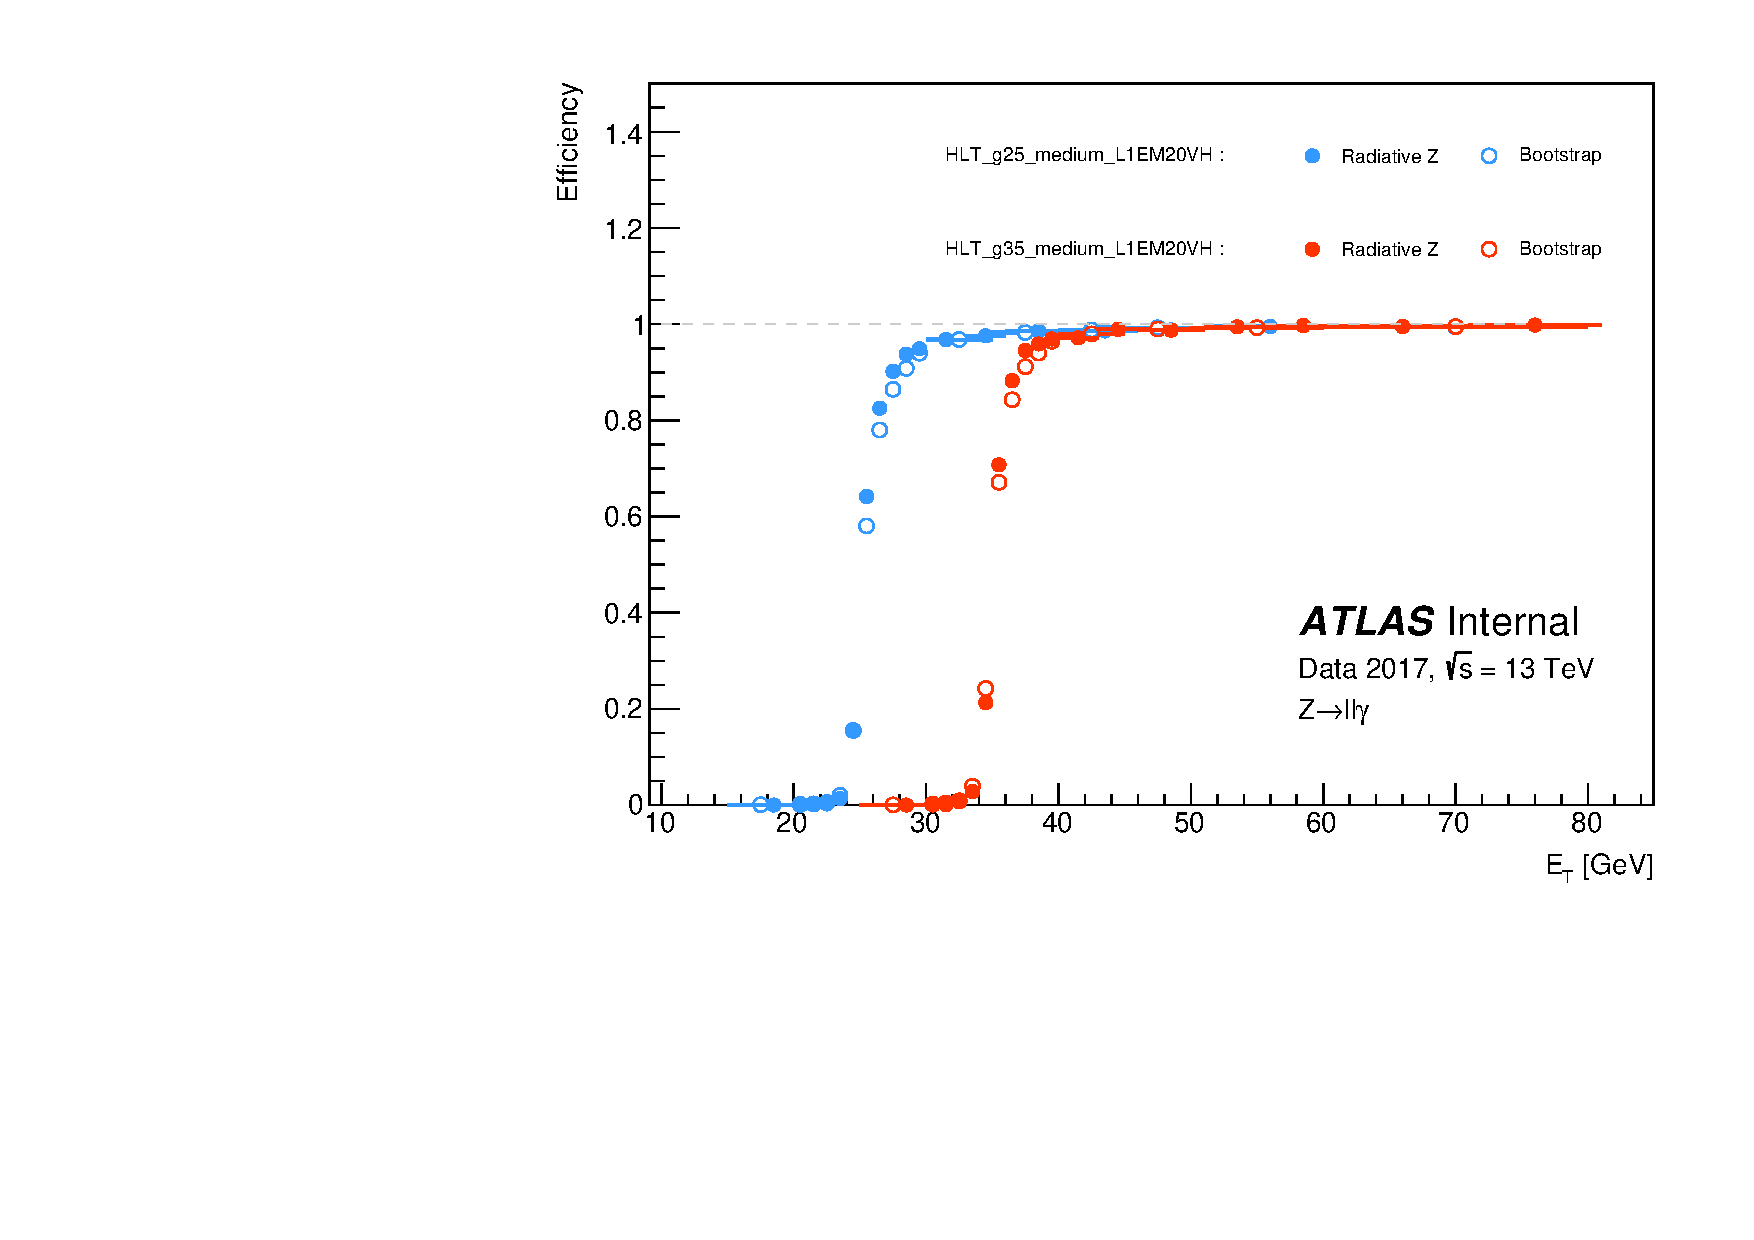
\includegraphics[width=0.6\textwidth]{images/trigger/comp_eff_et_bootstrap.pdf}
	\caption{Comparación de las eficiencias utilizando el método Bootstrap y el método del bosón $Z$ radiativo para dos triggers del 2017.}
  \label{fig:bs_vs_zrad}
\end{figure}


La incerteza estadística para las eficiencias se obtiene como el intervalo de confianza de un estimador de Bayes con el método de Jeffrey \cite{Casadei_2012}.
Las incertezas sistemáticas se obtienen a partir de las variaciones en las eficiencias al modificar algunas de las selecciones empleadas en el método, principalmente las asociadas a los leptones para evitar un posible sesgo en esa selección. El requisito sobre las masas invariantes se varió de $36\,\gev<m_{ll}<87\,\gev$ a $44\,\gev<m_{ll}<79\,\gev$, y de 
$82\,\gev<m_{ll\gamma}<100\,\gev$ a $88\,\gev<m_{ll\gamma}<94\,\gev$, y se modificó el requerimiento de identificación de los leptones a \texttt{Tight} y \texttt{Medium}, y el de aislamiento a \texttt{FixedCutTight}. En general las incertezas totales tomaban valores menores al 10\%.





\begin{figure}[!htpb]
  \centering
      {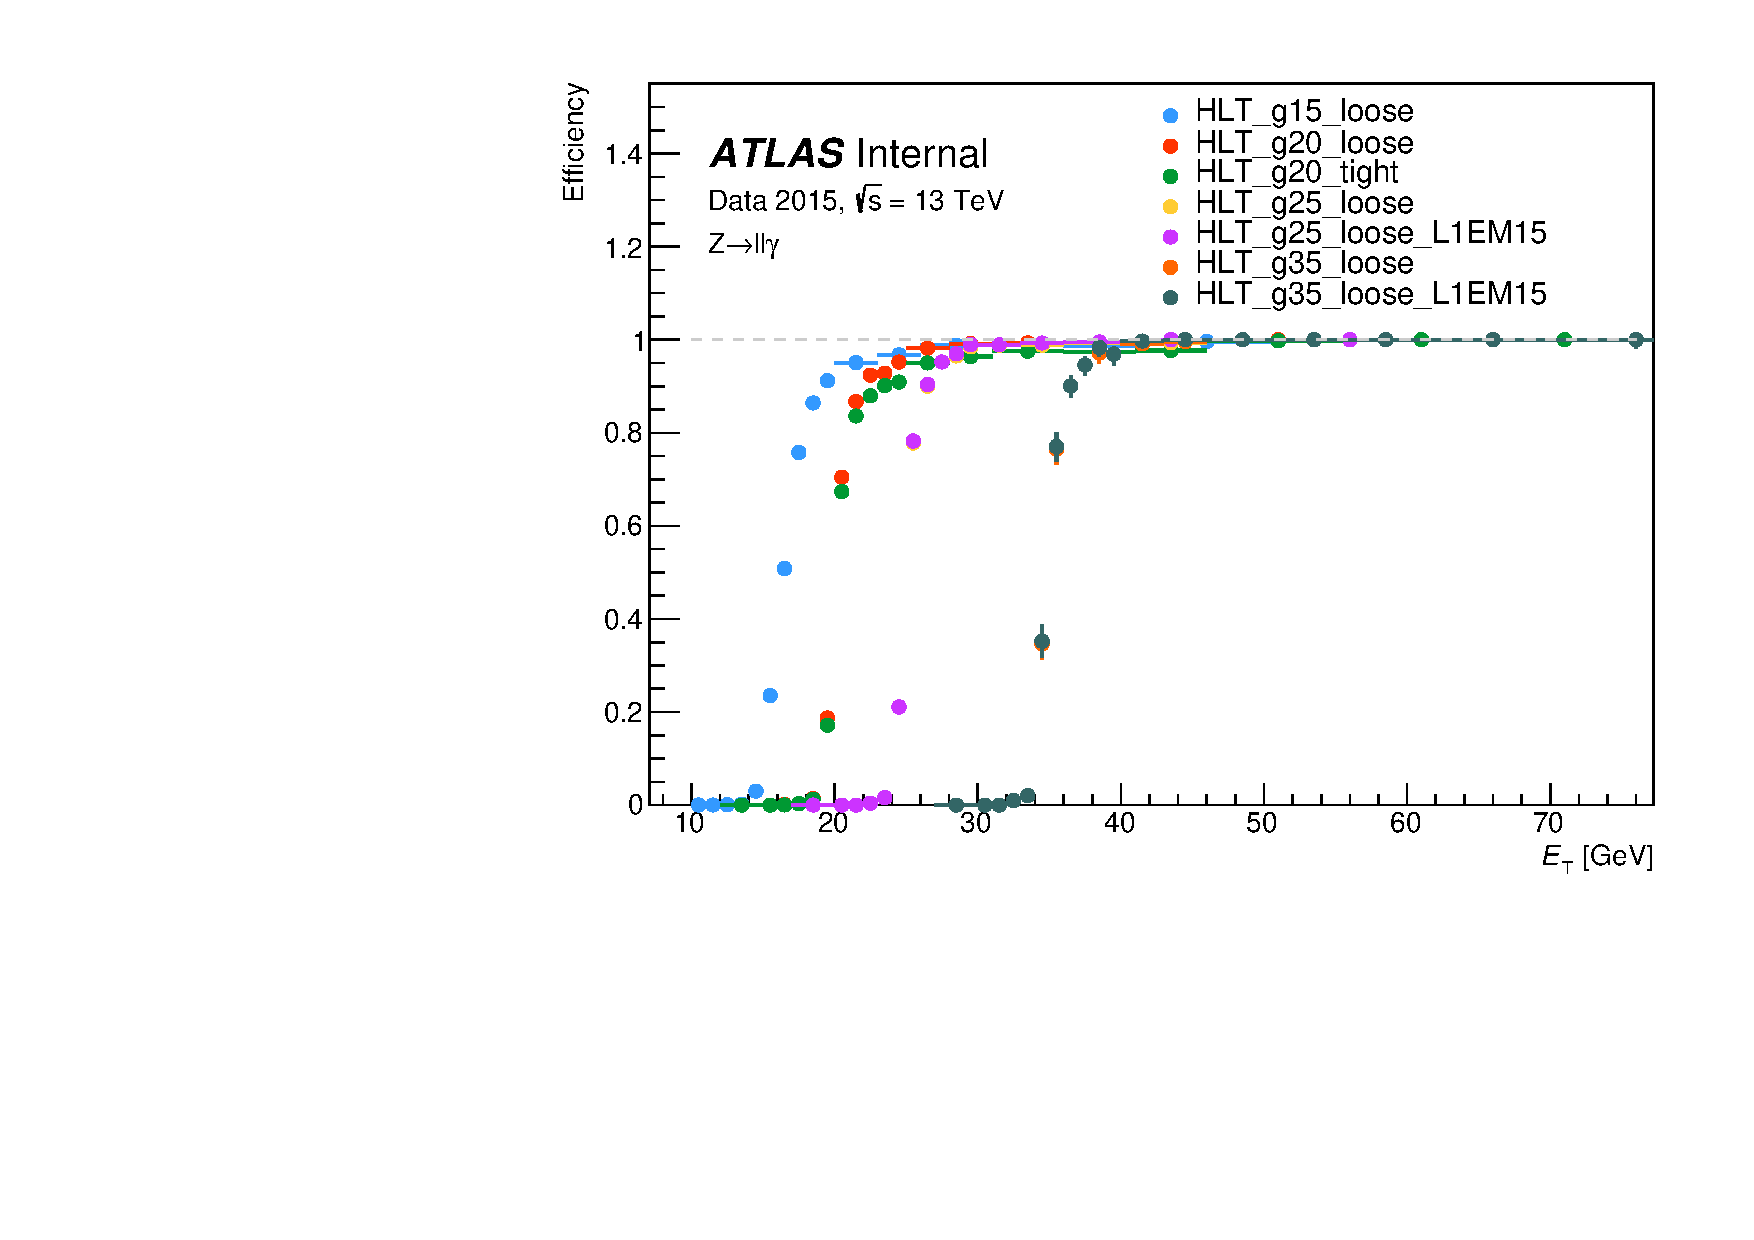
\includegraphics[width=0.30\textwidth]{images/trigger/2015_eff_et.pdf}}
      {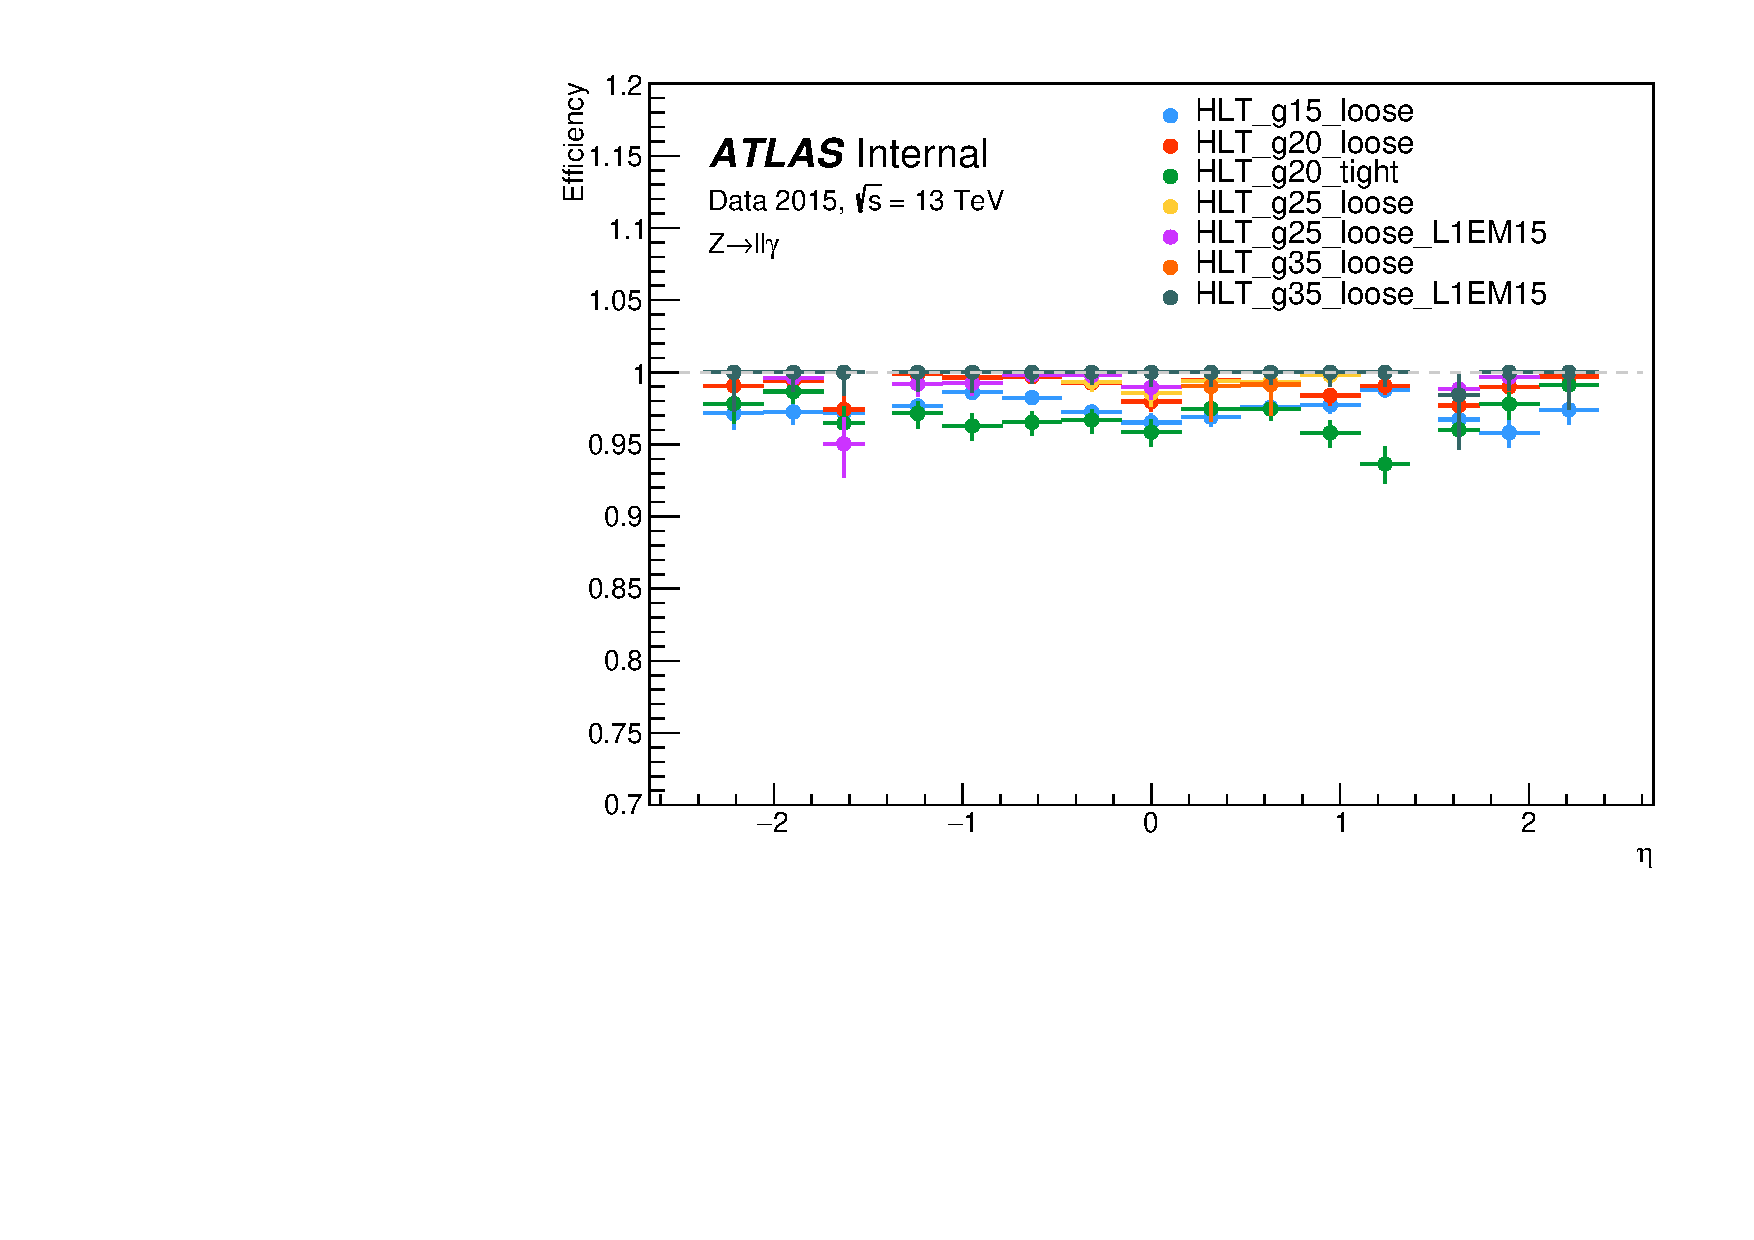
\includegraphics[width=0.30\textwidth]{images/trigger/2015_eff_eta_zoom.pdf}}
      {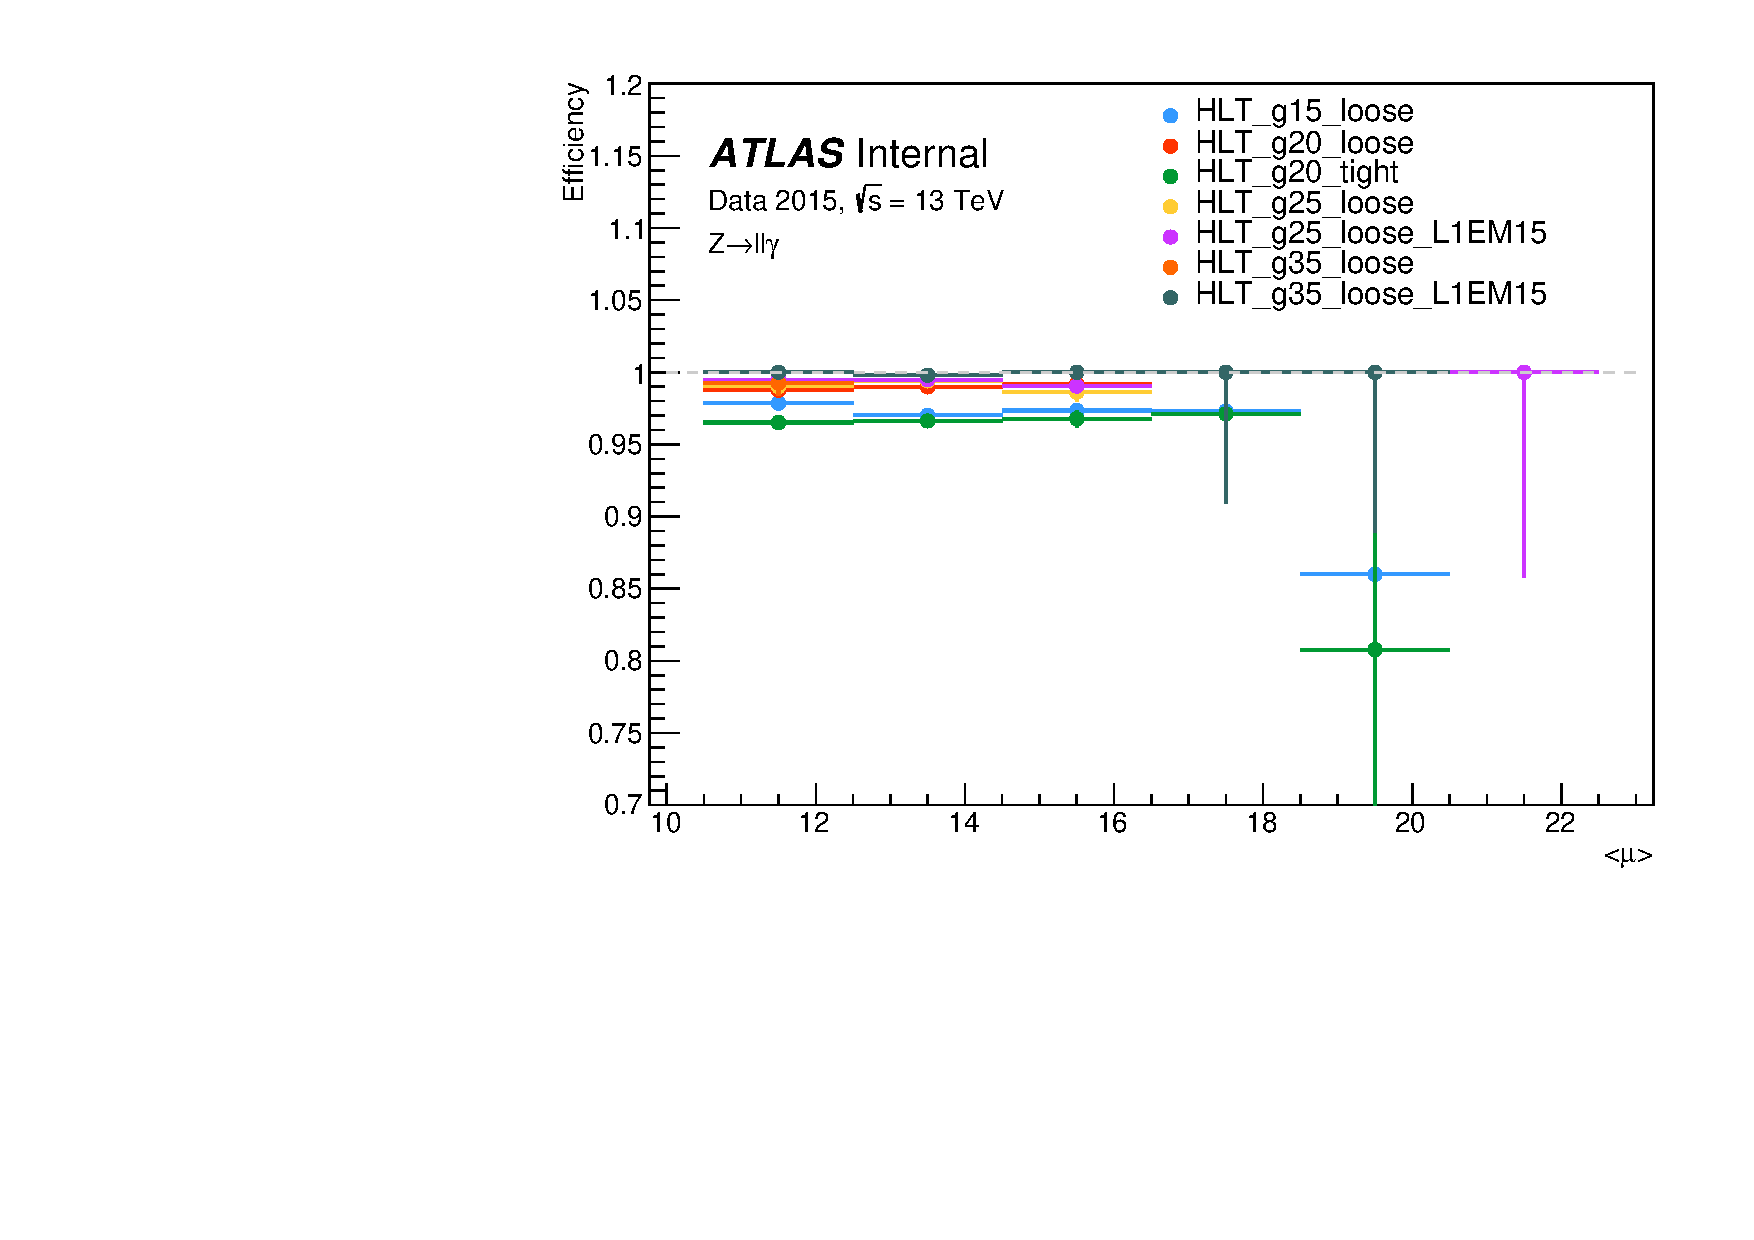
\includegraphics[width=0.30\textwidth]{images/trigger/2015_eff_mu_zoom.pdf}}
      \caption{Eficiencias de los triggers de fotones para el año 2015 en función del \ET (izquierda), $\eta$ (centro) y $\langle\mu\rangle$ (derecha).}
      \label{fig:photon_trig_eff_2015}
\end{figure}
\begin{figure}[!htpb]
  \centering
      {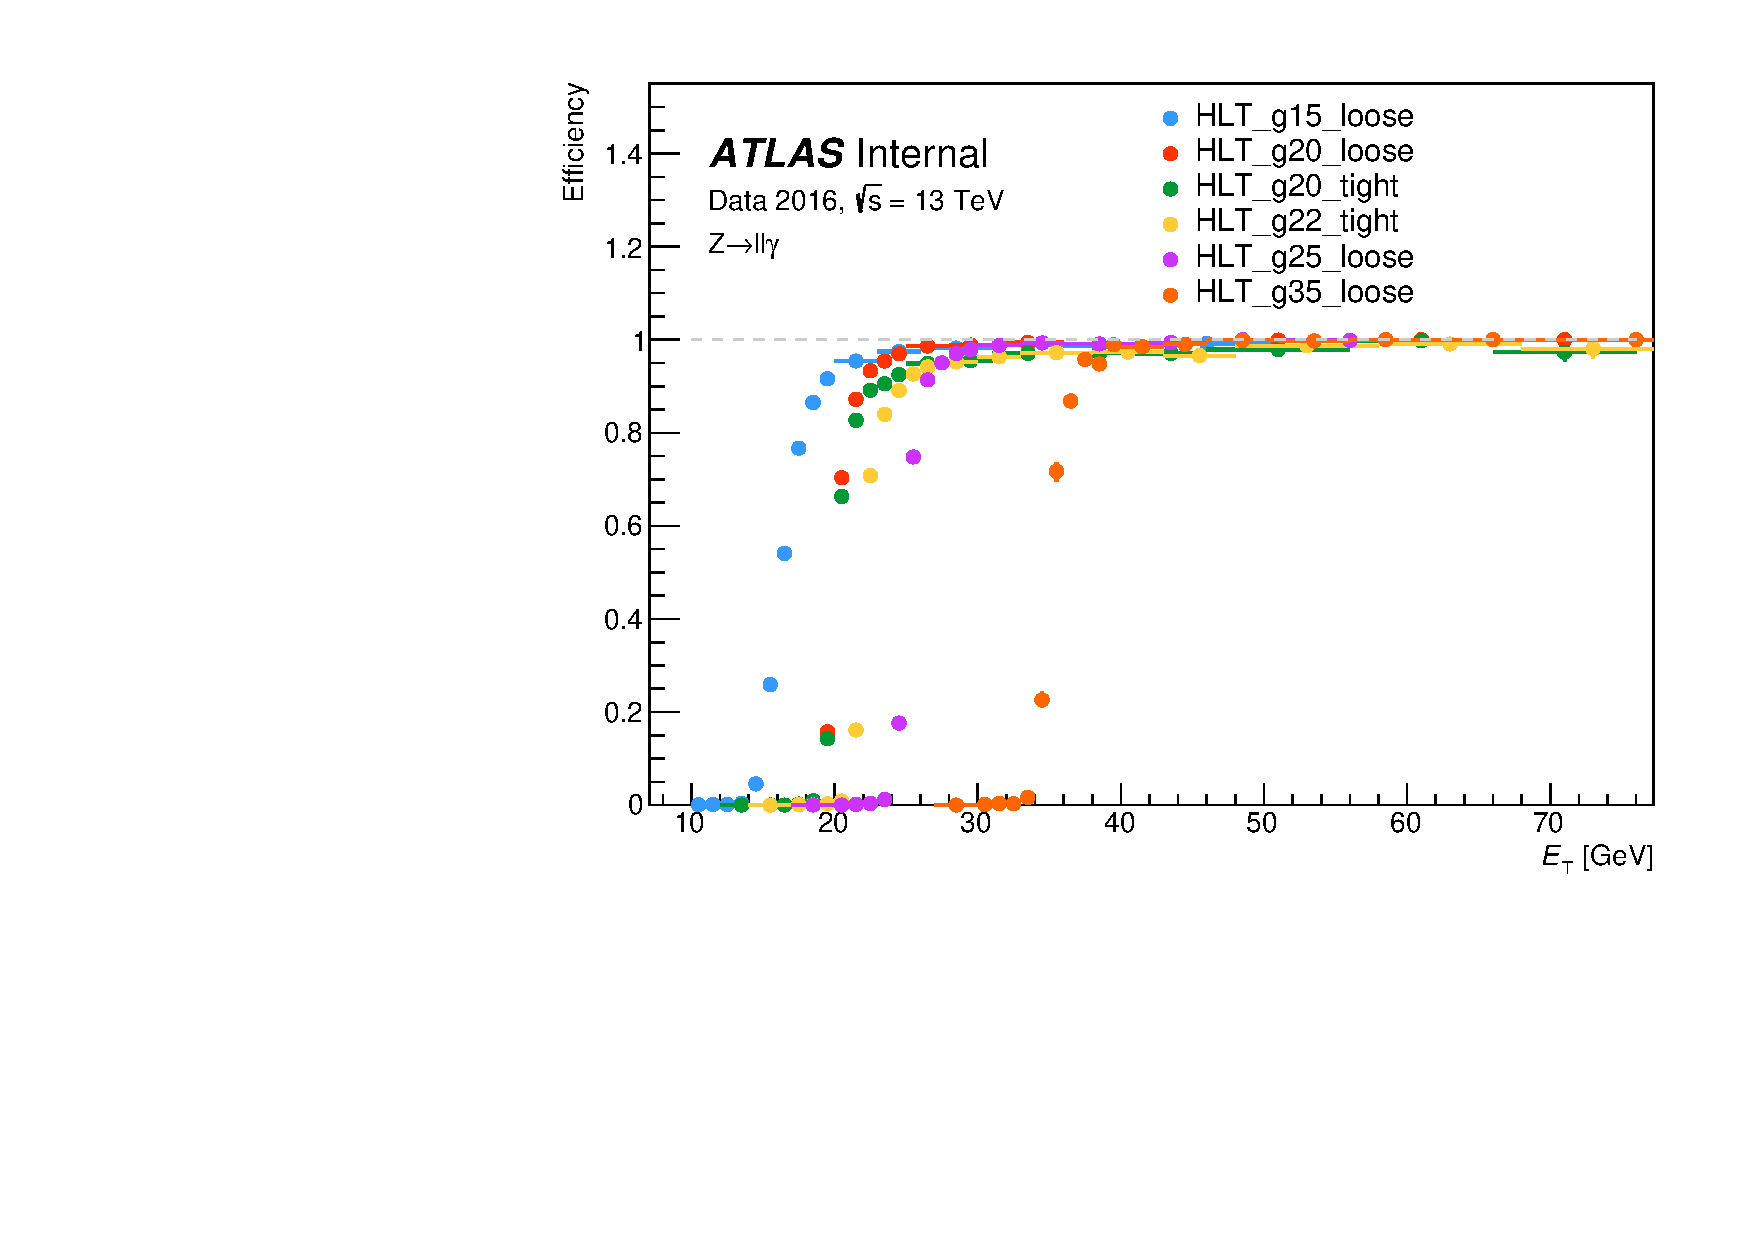
\includegraphics[width=0.30\textwidth]{images/trigger/2016_eff_et.pdf}}
      {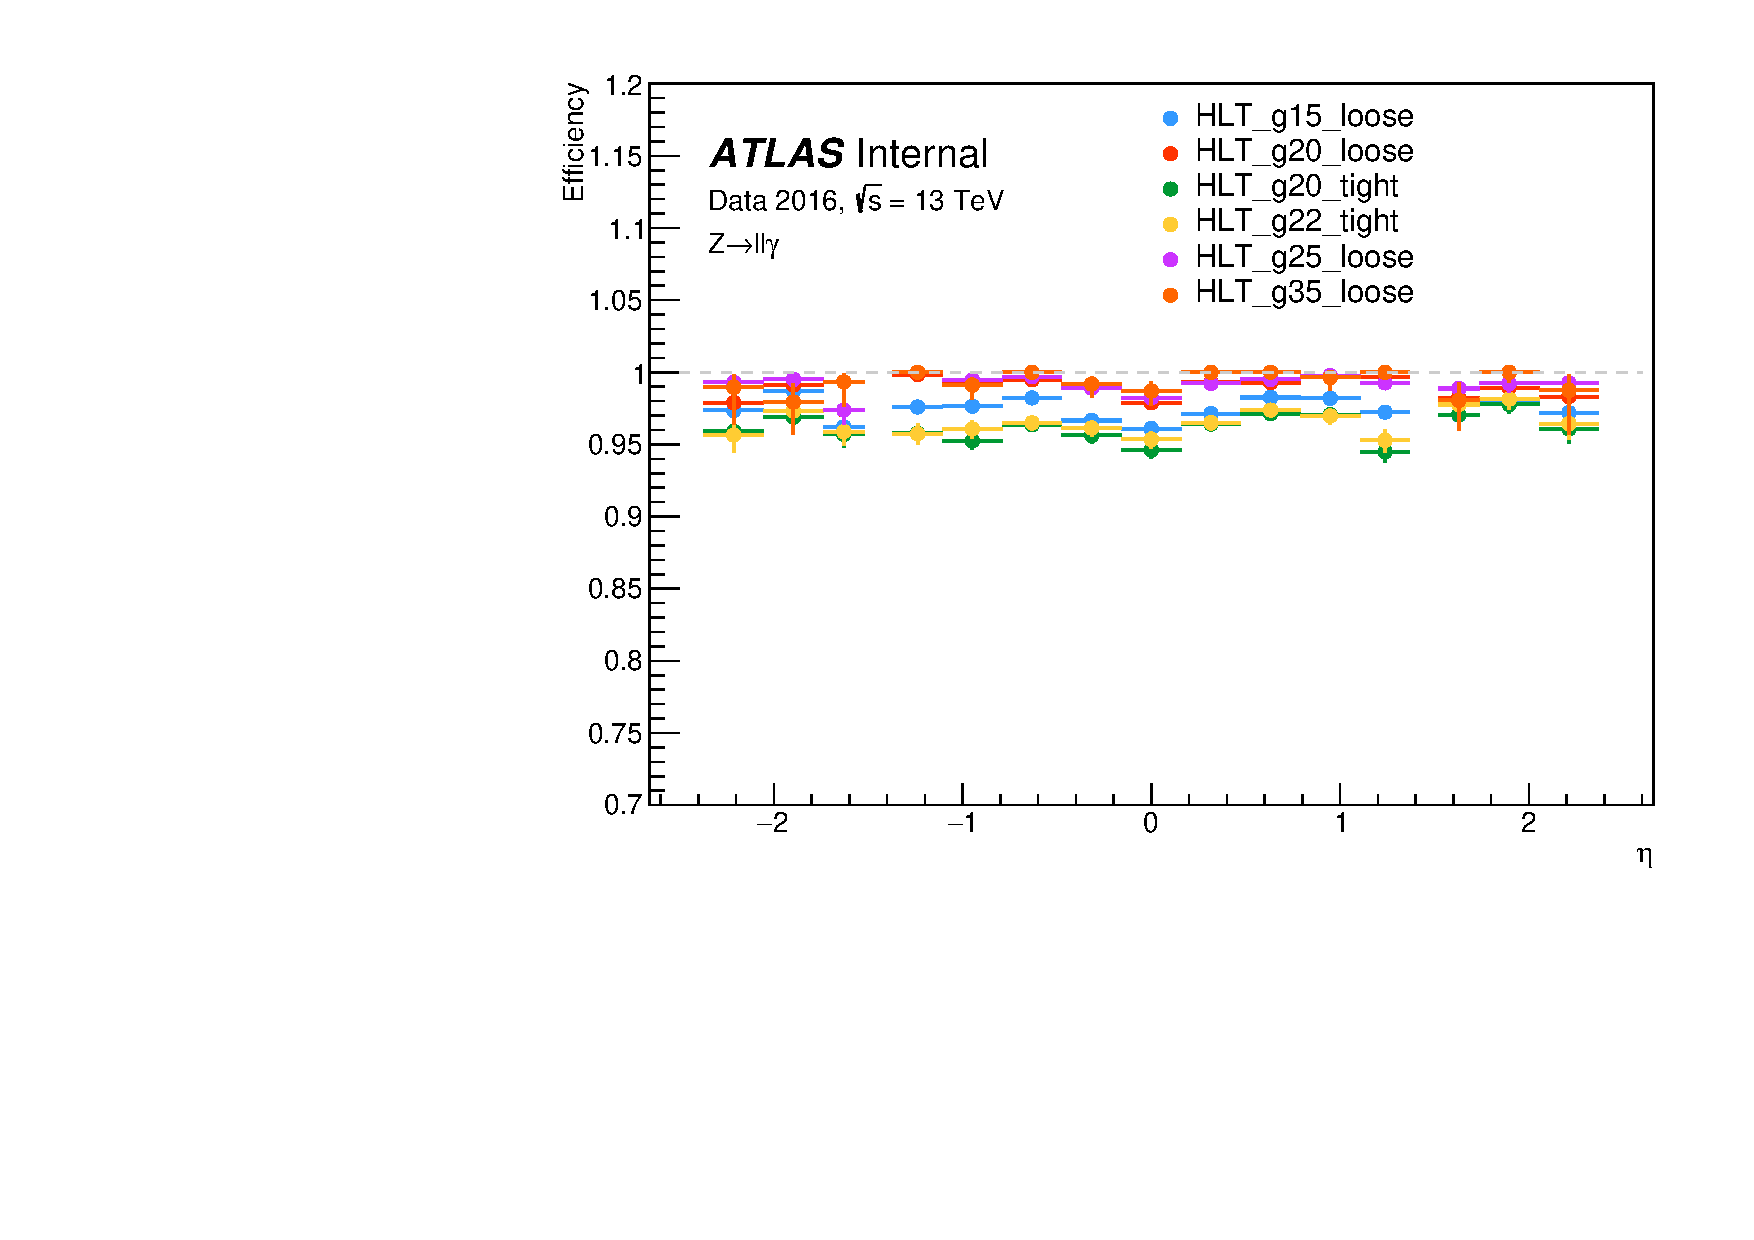
\includegraphics[width=0.30\textwidth]{images/trigger/2016_eff_eta_zoom.pdf}}
      {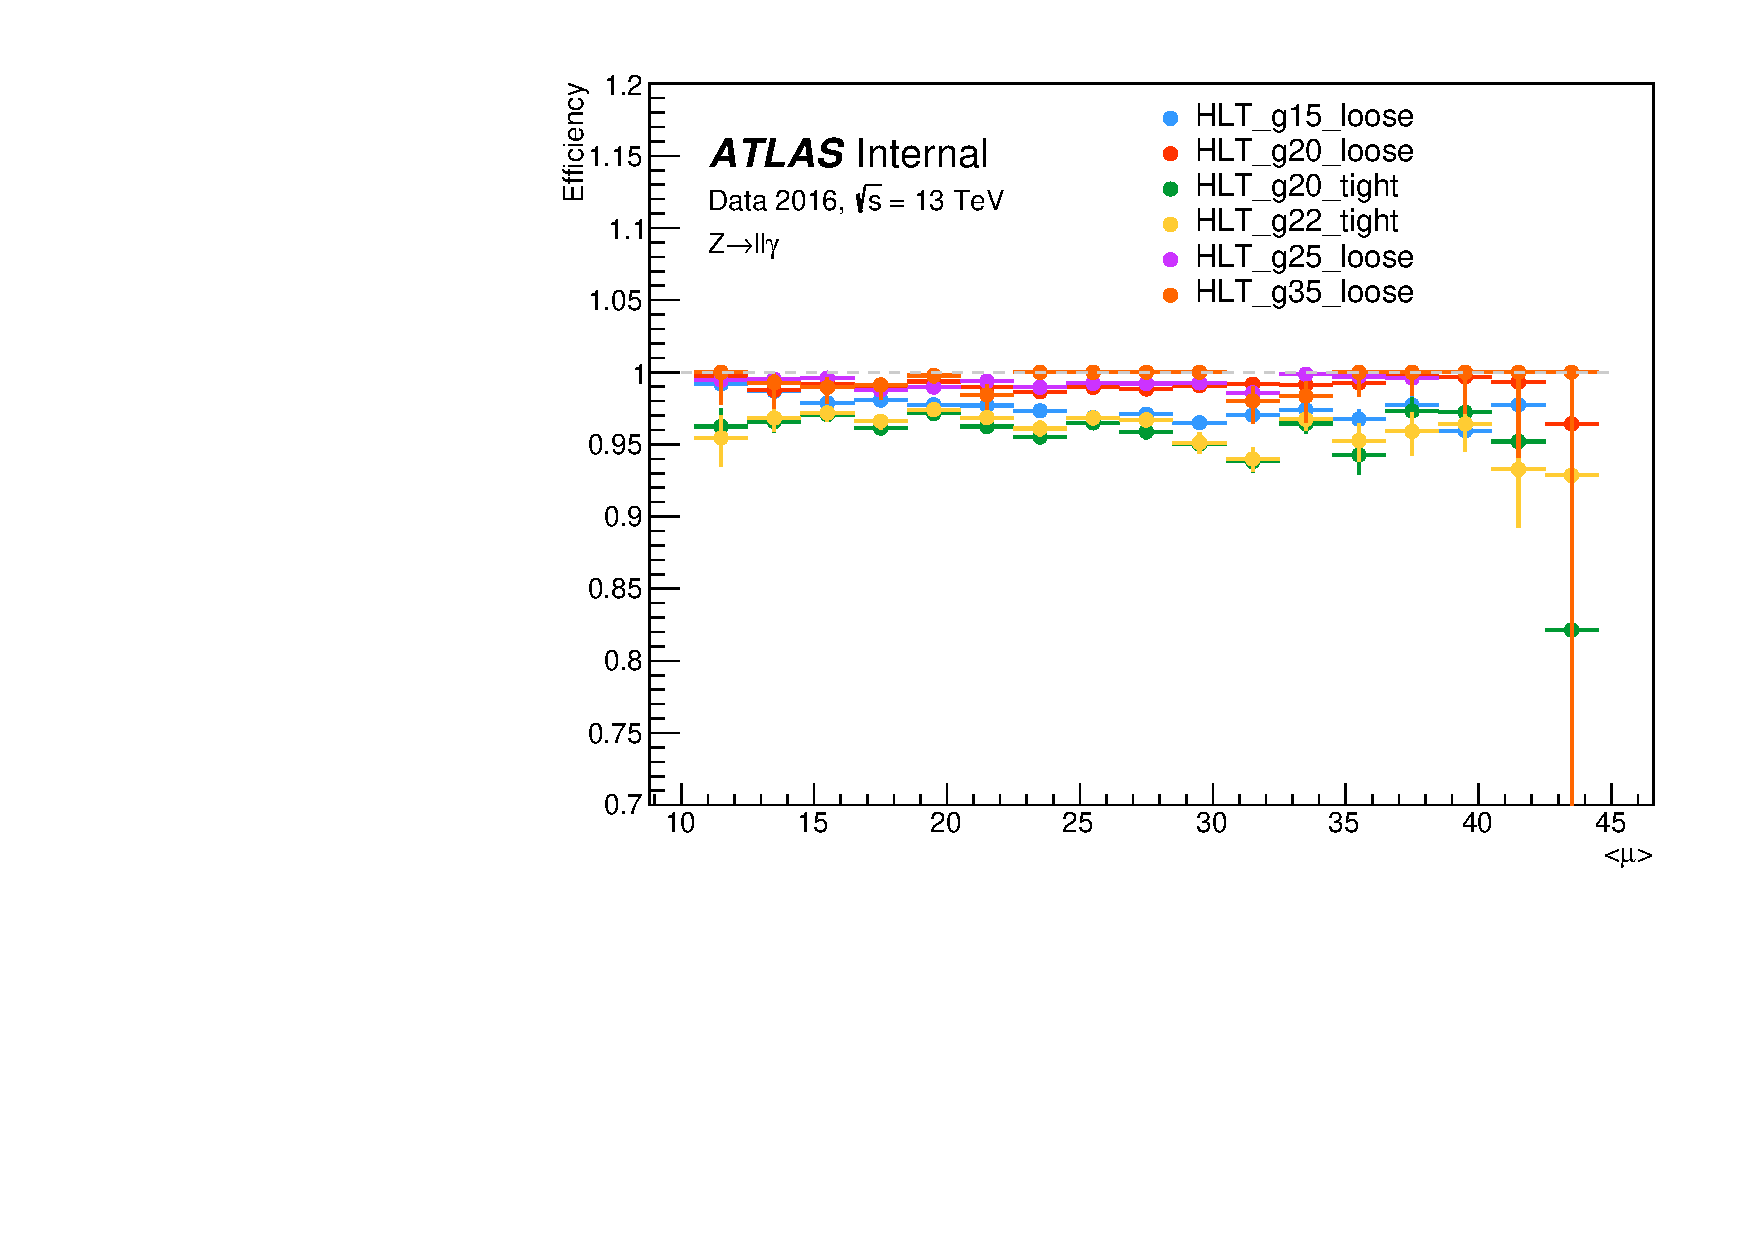
\includegraphics[width=0.30\textwidth]{images/trigger/2016_eff_mu_zoom.pdf}}
      \caption{Eficiencias de los triggers de fotones para el año 2016 en función del \ET (izquierda), $\eta$ (centro) y $\langle\mu\rangle$ (derecha).}
      \label{fig:photon_trig_eff_2016}
\end{figure}
\begin{figure}[!htpb]
  \centering
      {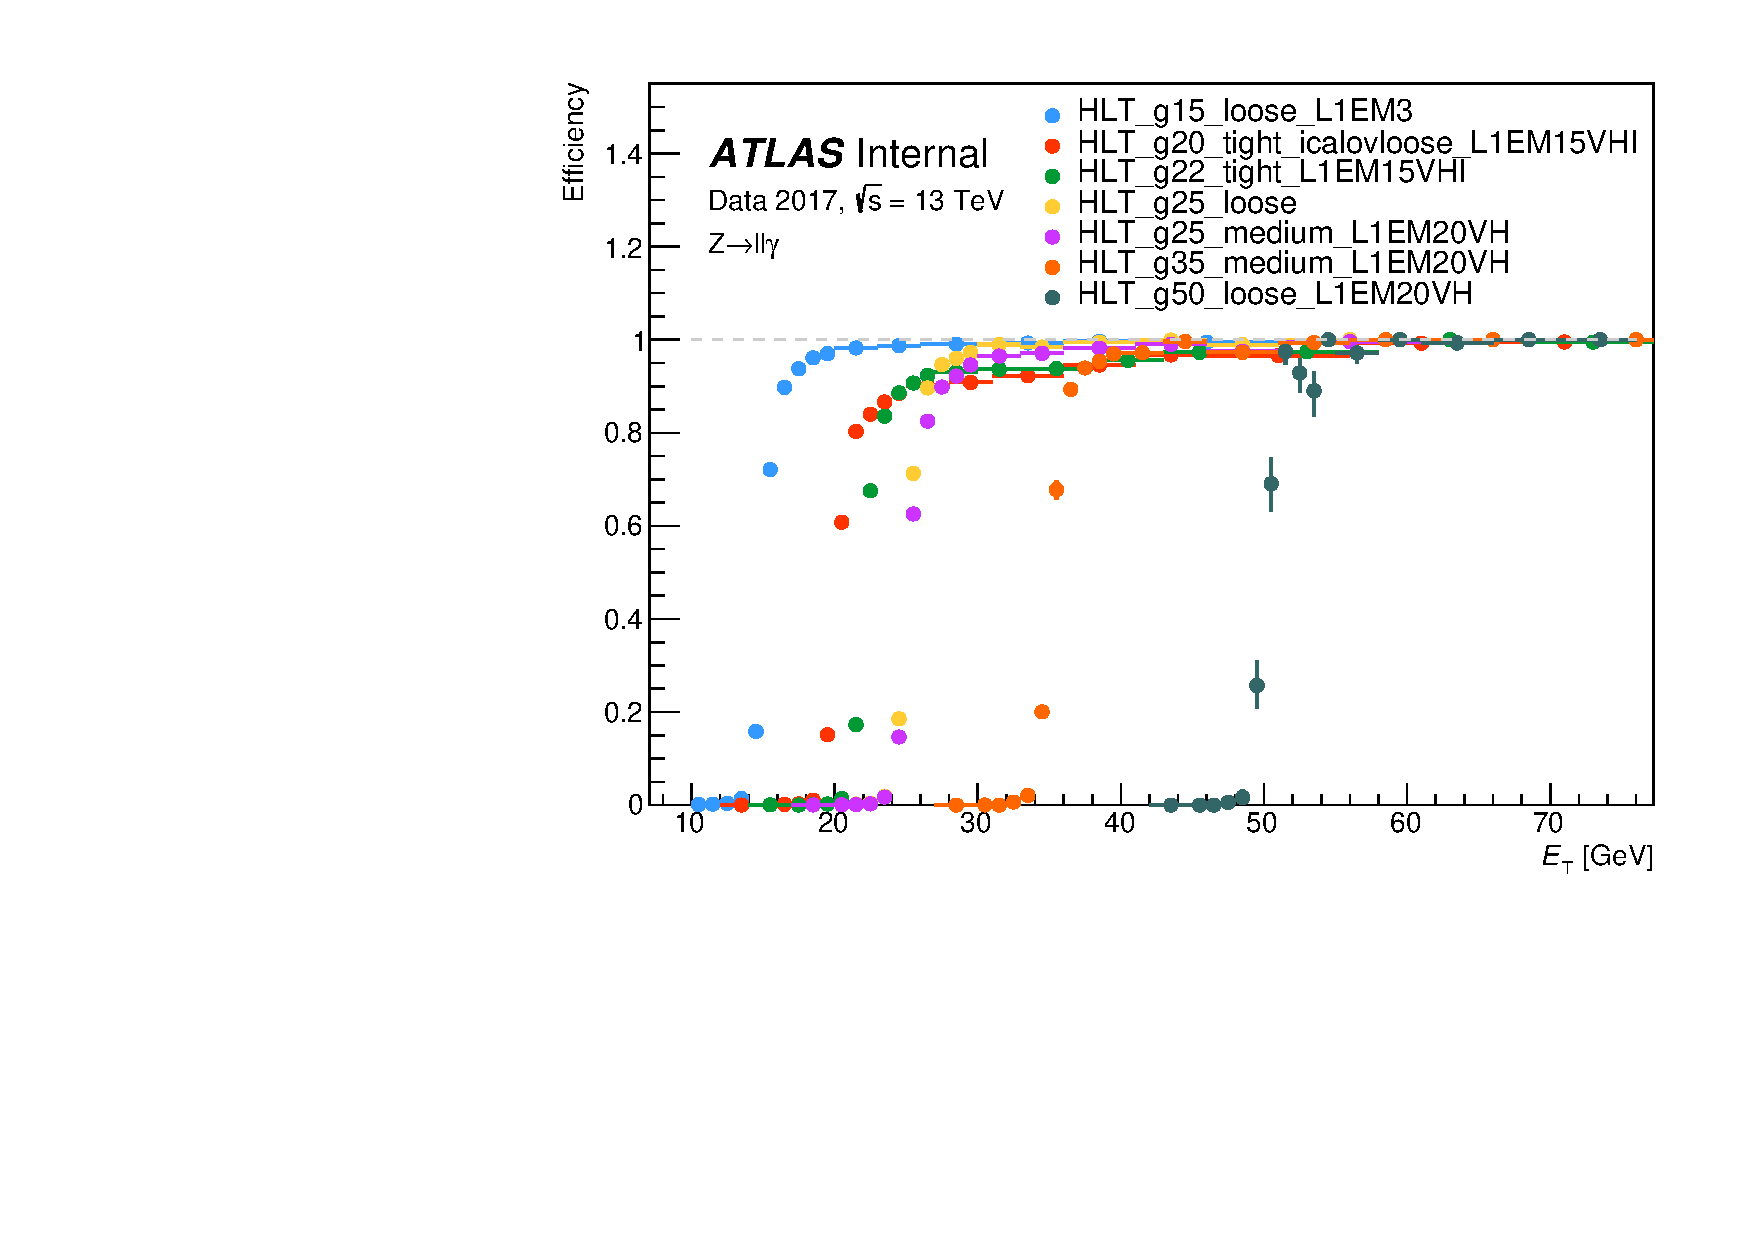
\includegraphics[width=0.30\textwidth]{images/trigger/2017_eff_et.pdf}}
      {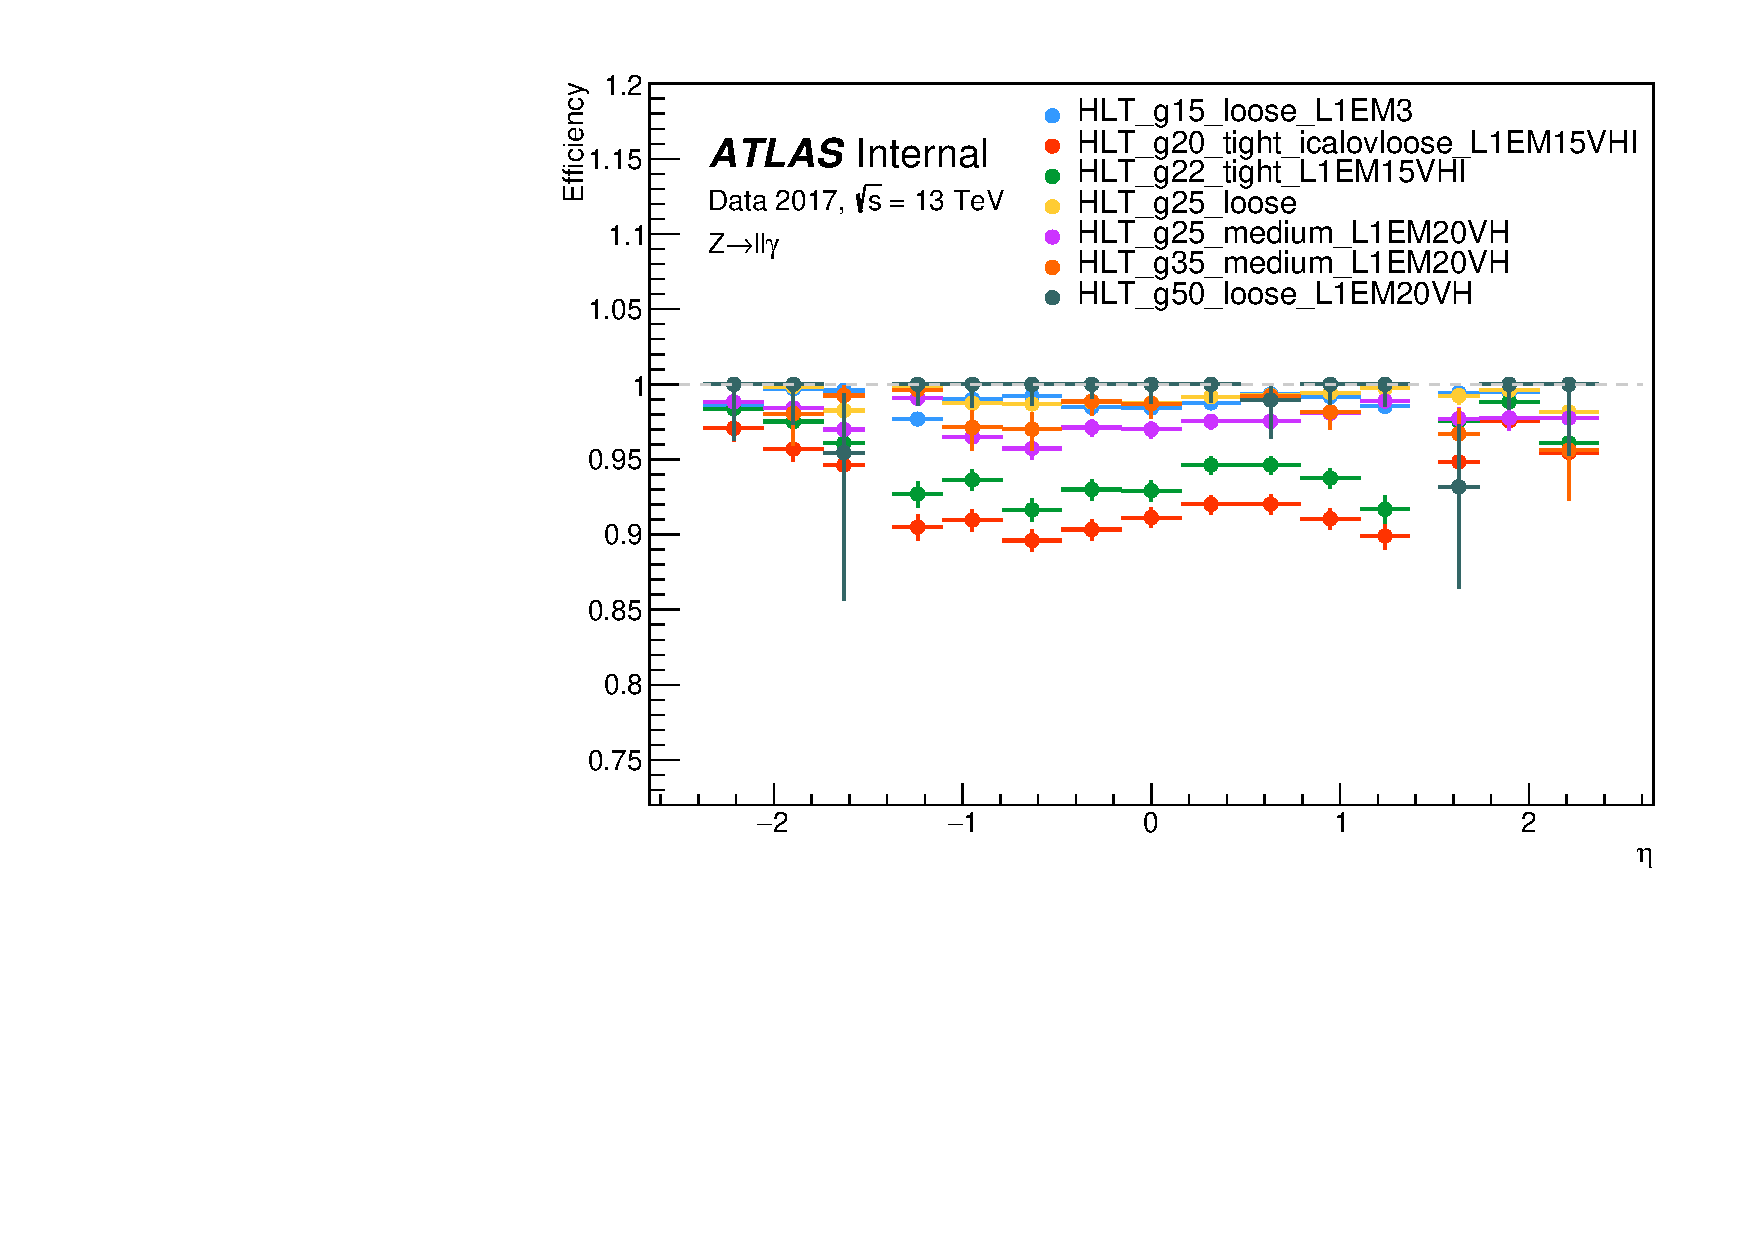
\includegraphics[width=0.30\textwidth]{images/trigger/2017_eff_eta_zoom.pdf}}
      {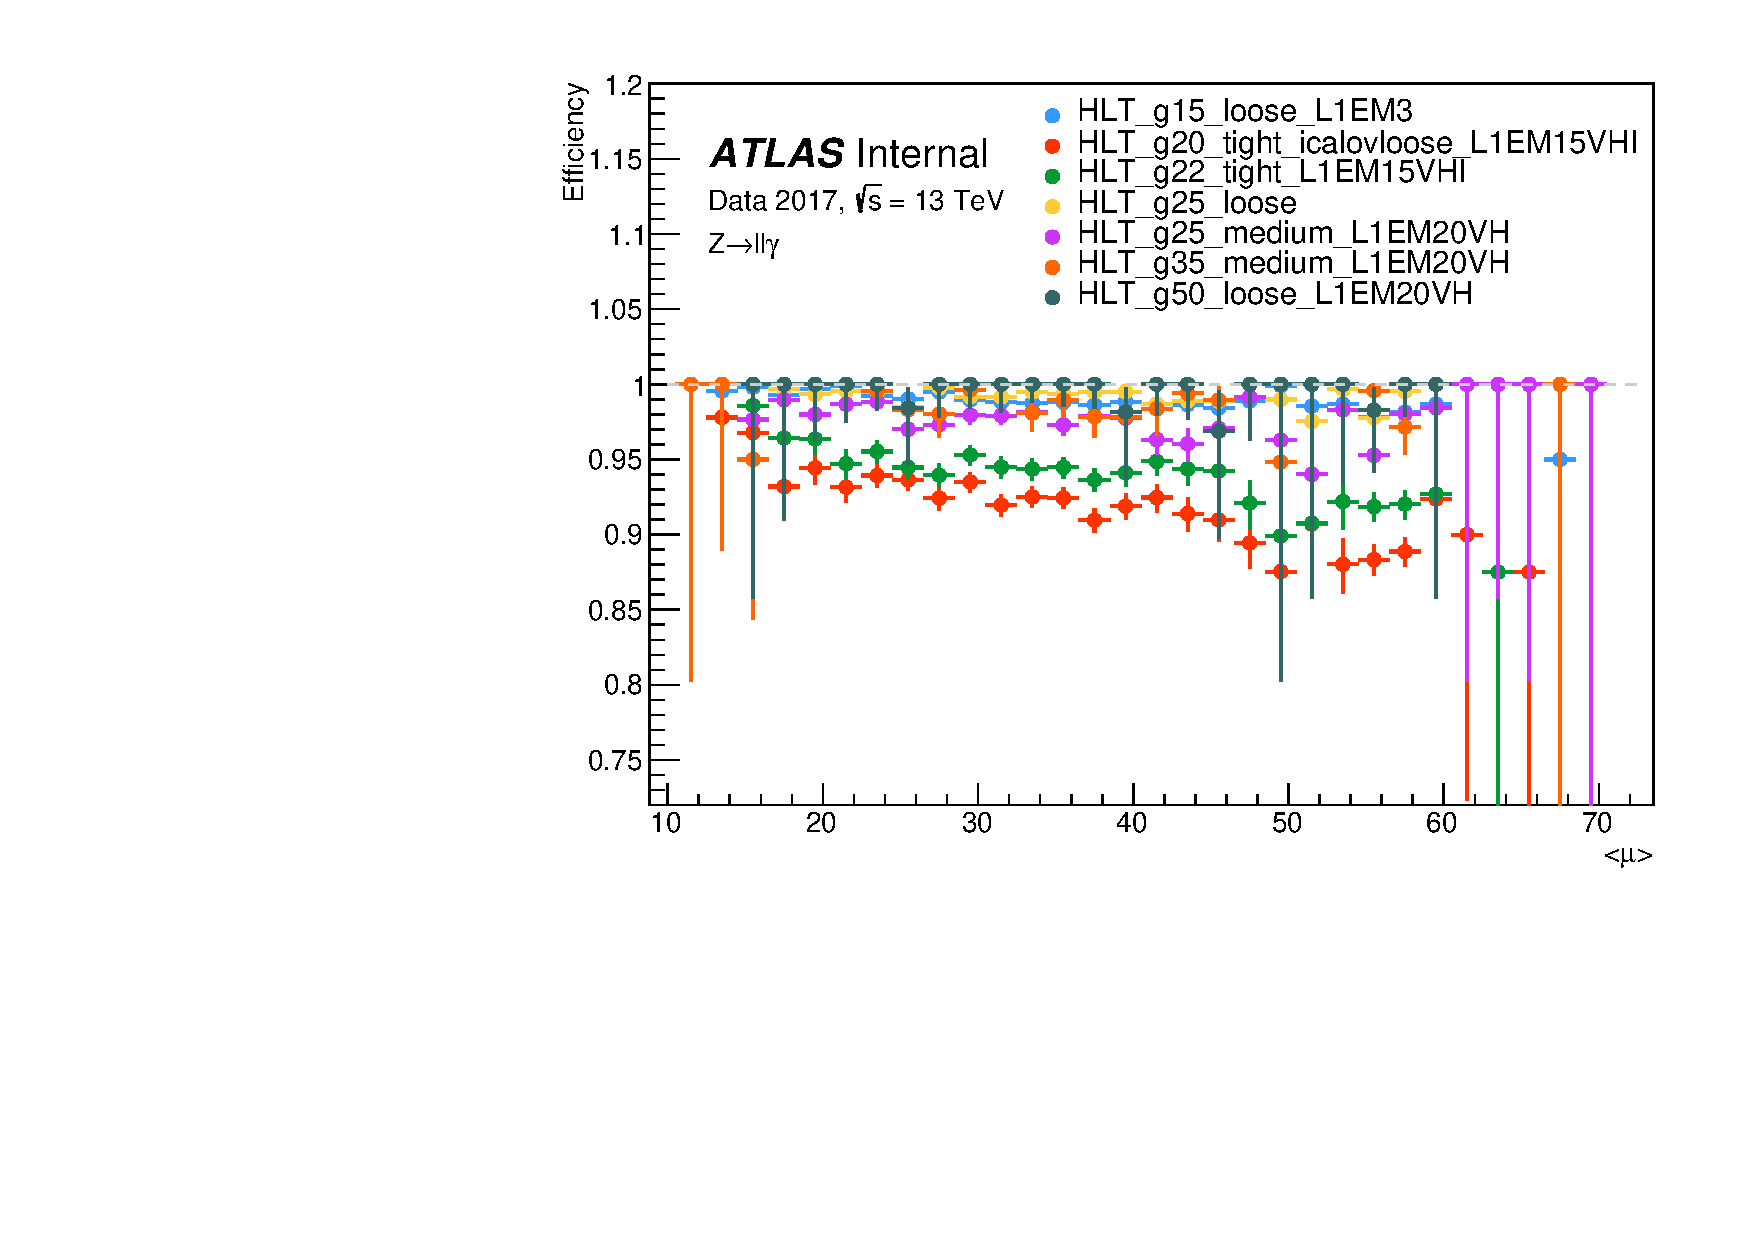
\includegraphics[width=0.30\textwidth]{images/trigger/2017_eff_mu_zoom.pdf}}
      \caption{Eficiencias de los triggers de fotones para el año 2017 en función del \ET (izquierda), $\eta$ (centro) y $\langle\mu\rangle$ (derecha).}
      \label{fig:photon_trig_eff_2017}
\end{figure}
\begin{figure}[!htpb]
  \centering
      {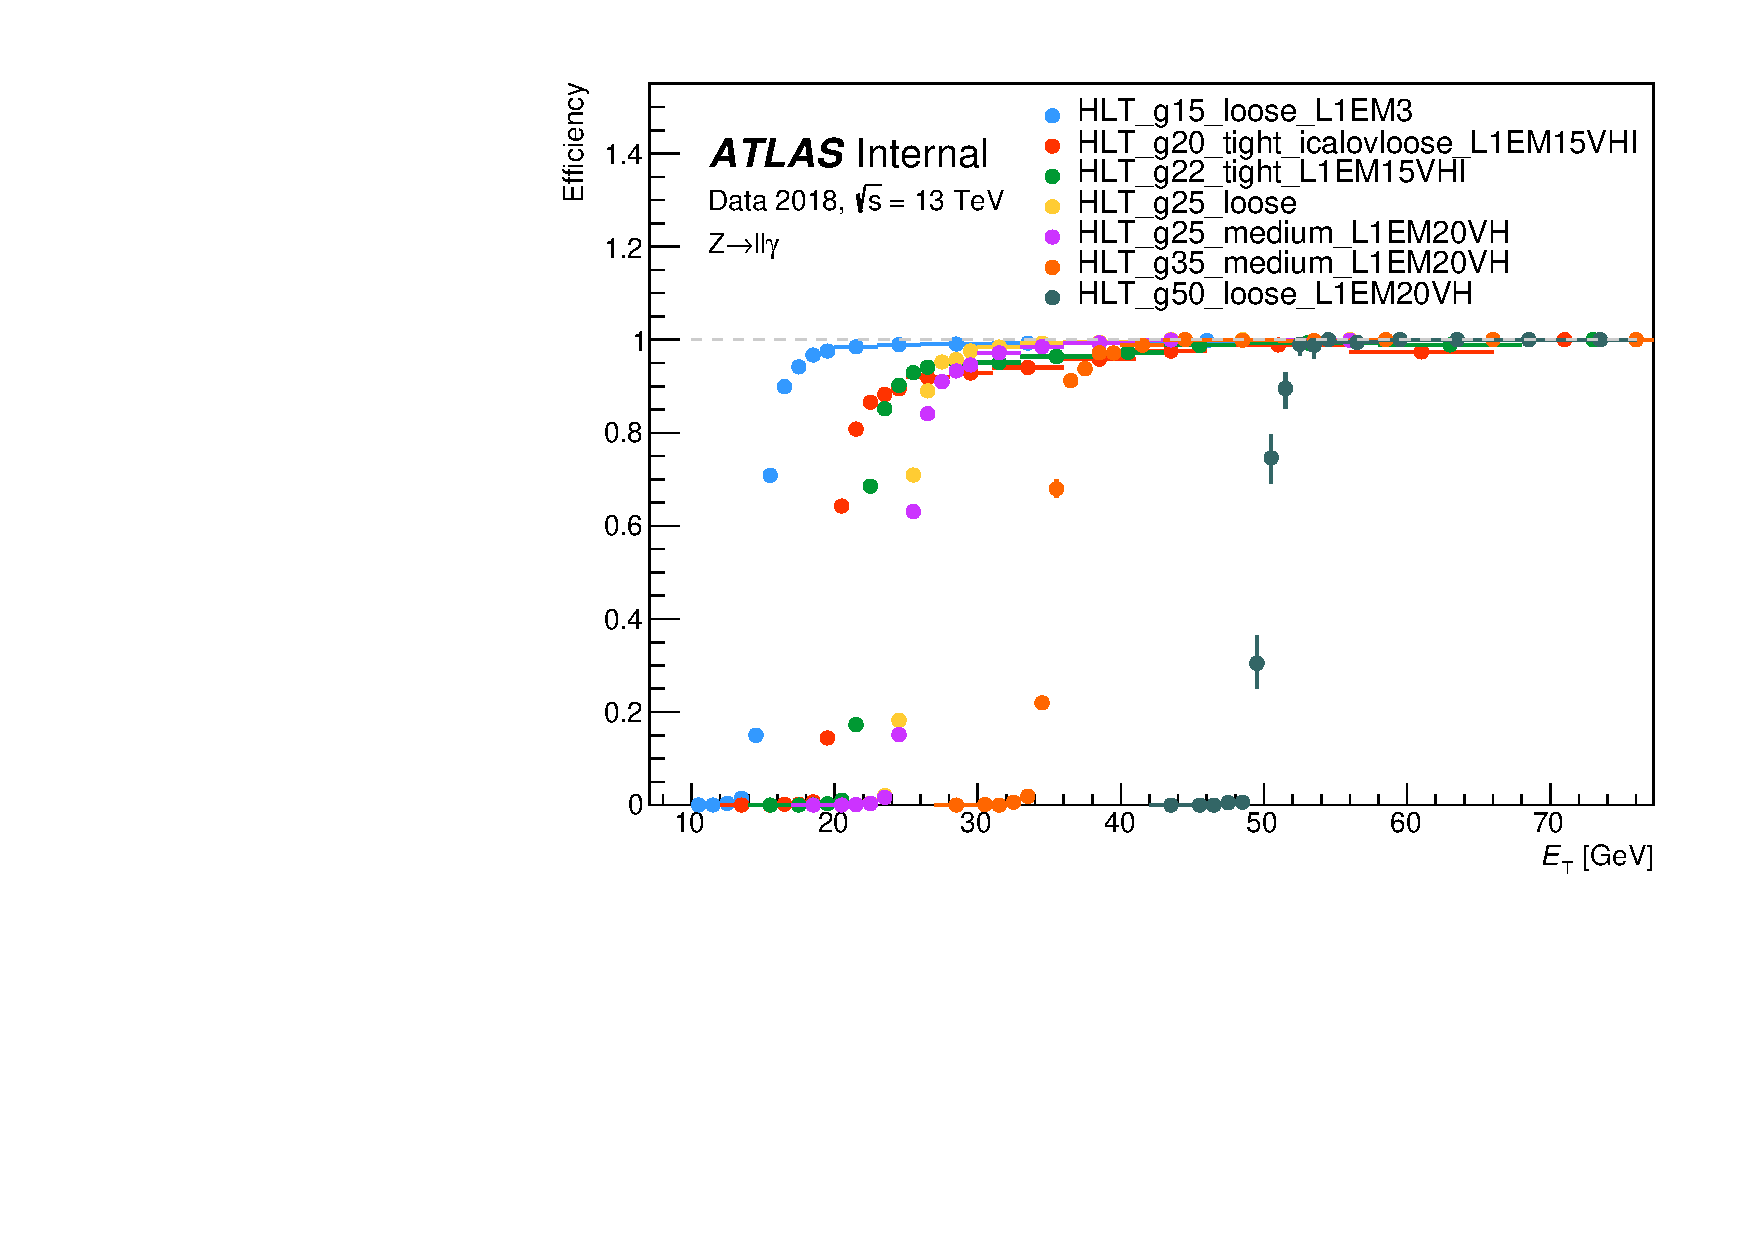
\includegraphics[width=0.30\textwidth]{images/trigger/2018_eff_et.pdf}}
      {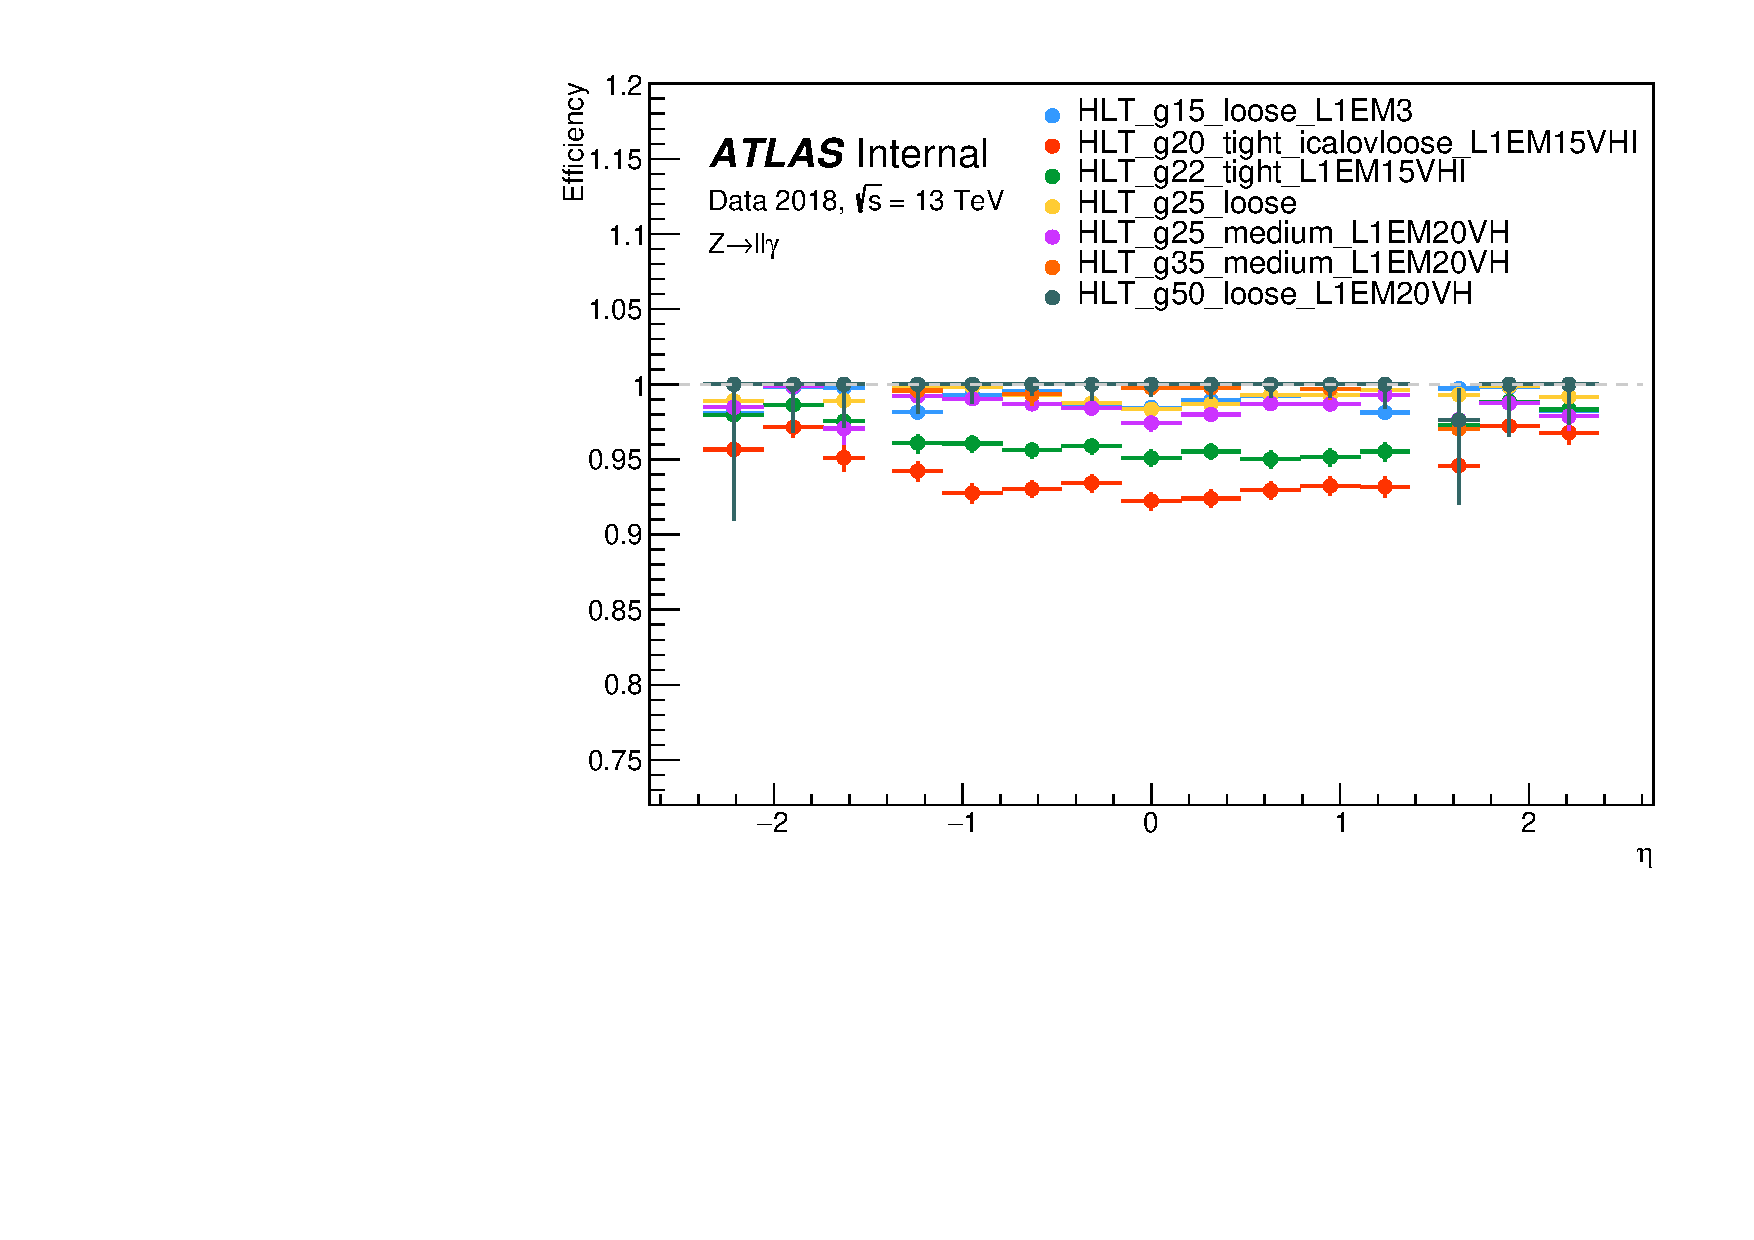
\includegraphics[width=0.30\textwidth]{images/trigger/2018_eff_eta_zoom.pdf}}
      {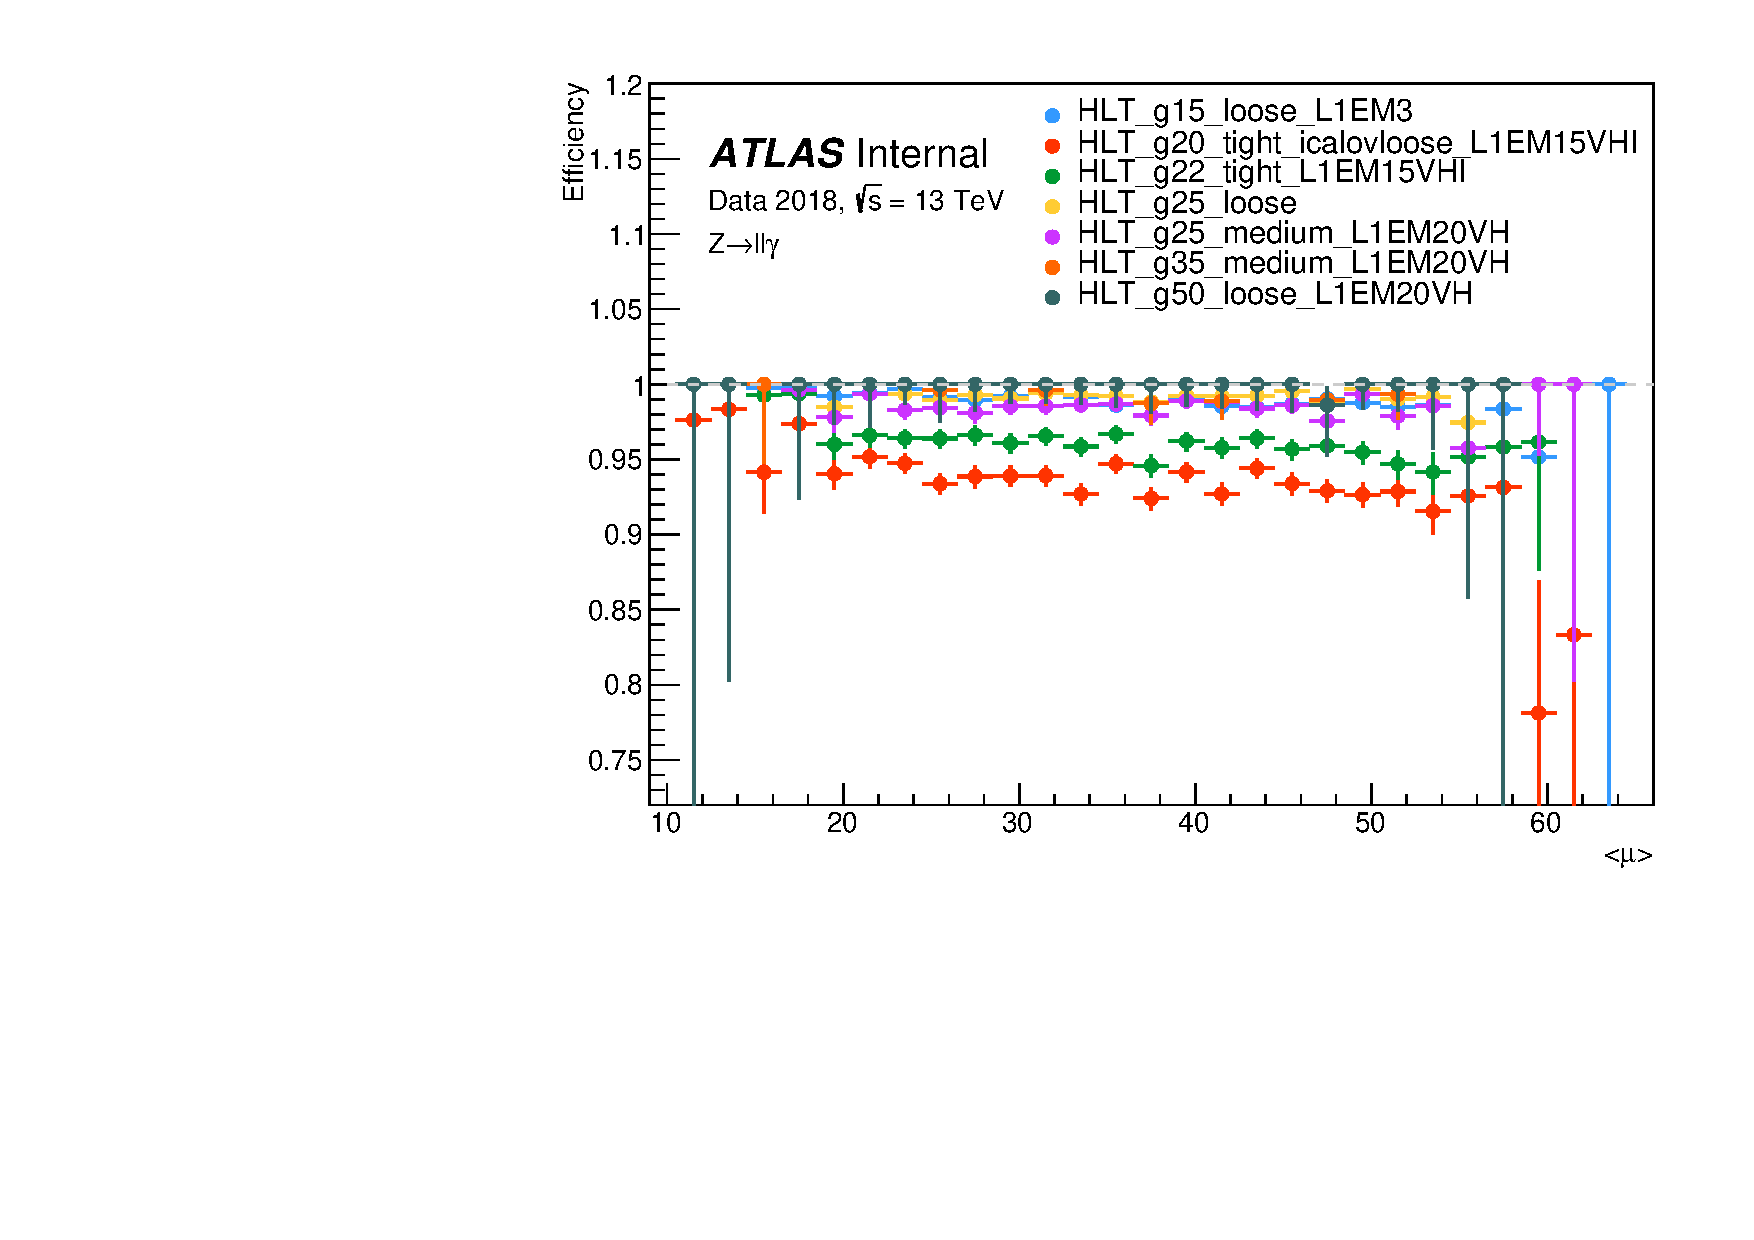
\includegraphics[width=0.30\textwidth]{images/trigger/2018_eff_mu_zoom.pdf}}
      \caption{Eficiencias de los triggers de fotones para el año 2018 en función del \ET (izquierda), $\eta$ (centro) y $\langle\mu\rangle$ (derecha).}
      \label{fig:photon_trig_eff_2018}
\end{figure}


\section{Factores de escala de las eficiencias}\label{sec:trig_sf}

Las simulaciones de Monte Carlo logran reproducir los procesos físicos en general con una alta precisión, pero naturalmente presentan imperfecciones principalmente relacionadas con la simulación de la interacción de las partículas con el material del detector. Estos efectos se traducen en eficiencias distintas (en general más altas) que las respectivas producidas en datos. Con el objetivo de corregir las simulaciones y que se asemejen lo más posible a los datos se calculan los Factores de Escala (SF), que son factores multiplicativos (pesos) aplicados luego a cada evento simulado según corresponda. Para el caso de la eficiencia del trigger de fotones, los SFs se definen como el cociente entre las eficiencias calculadas en datos y las calculadas con simulaciones:

\begin{equation}
	\text{SF}(\pt, \eta) = \frac{\epsilon^{\text{(datos)}}(\pt, \eta)}{\epsilon^{\text{(MC)}}(\pt, \eta)}
\end{equation}

Las eficiencias del trigger para simulaciones se calculan de la misma forma que en datos, pero utilizando simulaciones con procesos de producción de bosones $Z$ decayendo a electrones o muones, los cuales pueden irradiar un fotón. Los SFs con calculados para los mismos triggers que se calculó la eficiencia listados en la Tabla \ref{tab:trigg_eff}, en bines de \ET y $\eta$ simultáneamente y para distintos WPs de aislamiento. Las incertezas son calculadas directamente propagando las incertezas de ambos términos del cociente. Para valores de alto \ET el valor del SF es extrapolado a partir de los bines de bajo \ET, donde el método del bosón $Z$ radiativo tiene validez. En la región con \ET menor al umbral y en la región del crack, donde las eficiencias son prácticamente nulas, se fijan los SFs igual $1\pm1$. 
 
En las Figuras \ref{fig:SFs_2015_2016} y \ref{fig:SFs_2017_2018} se observan algunos de los SFs calculados para triggers de distintos años con WPs de aislamiento \texttt{FixedCutTightCaloOnly}. 
En todos los casos los SFs son muy cercanos a la unidad, lo que deja en evidencia el buen diseño y construcción del sistema de trigger y las simulaciones. Tanto las eficiencias como los factores de escala obtenidos en este trabajo son utilizados actualmente por todos los análisis de la colaboración ATLAS que utilicen una selección de datos con triggers de fotones del Run 2.

% \solved{Tanto para eficiencias como para SF, debería mencionar la tabla con los triggers para los cuales se calcularon?} Done!

\begin{figure}[!htpb]
  \centering
      {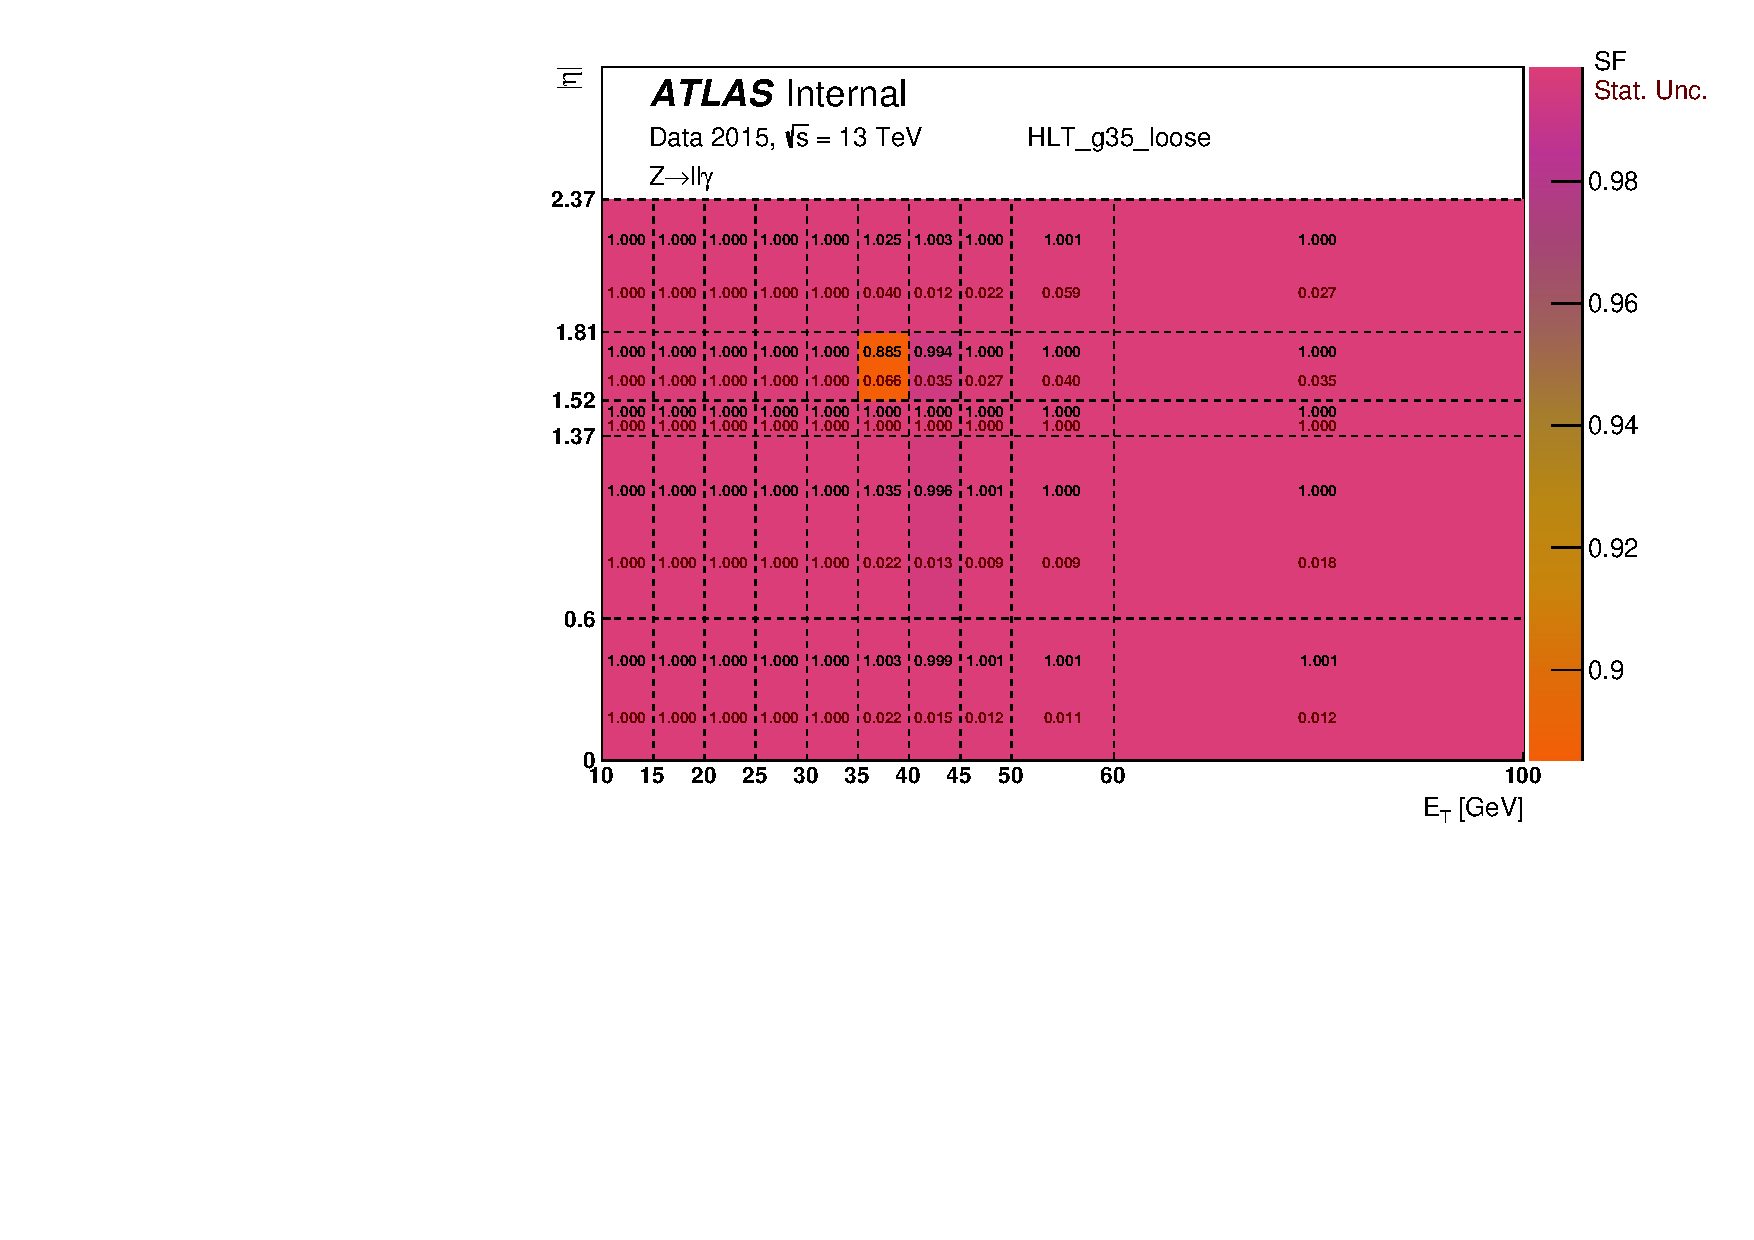
\includegraphics[width=0.45\textwidth]{images/trigger/2015_h_sf_et_eta_tr_HLT_g35_loose_FixedCutTightCaloOnly.pdf}}
      {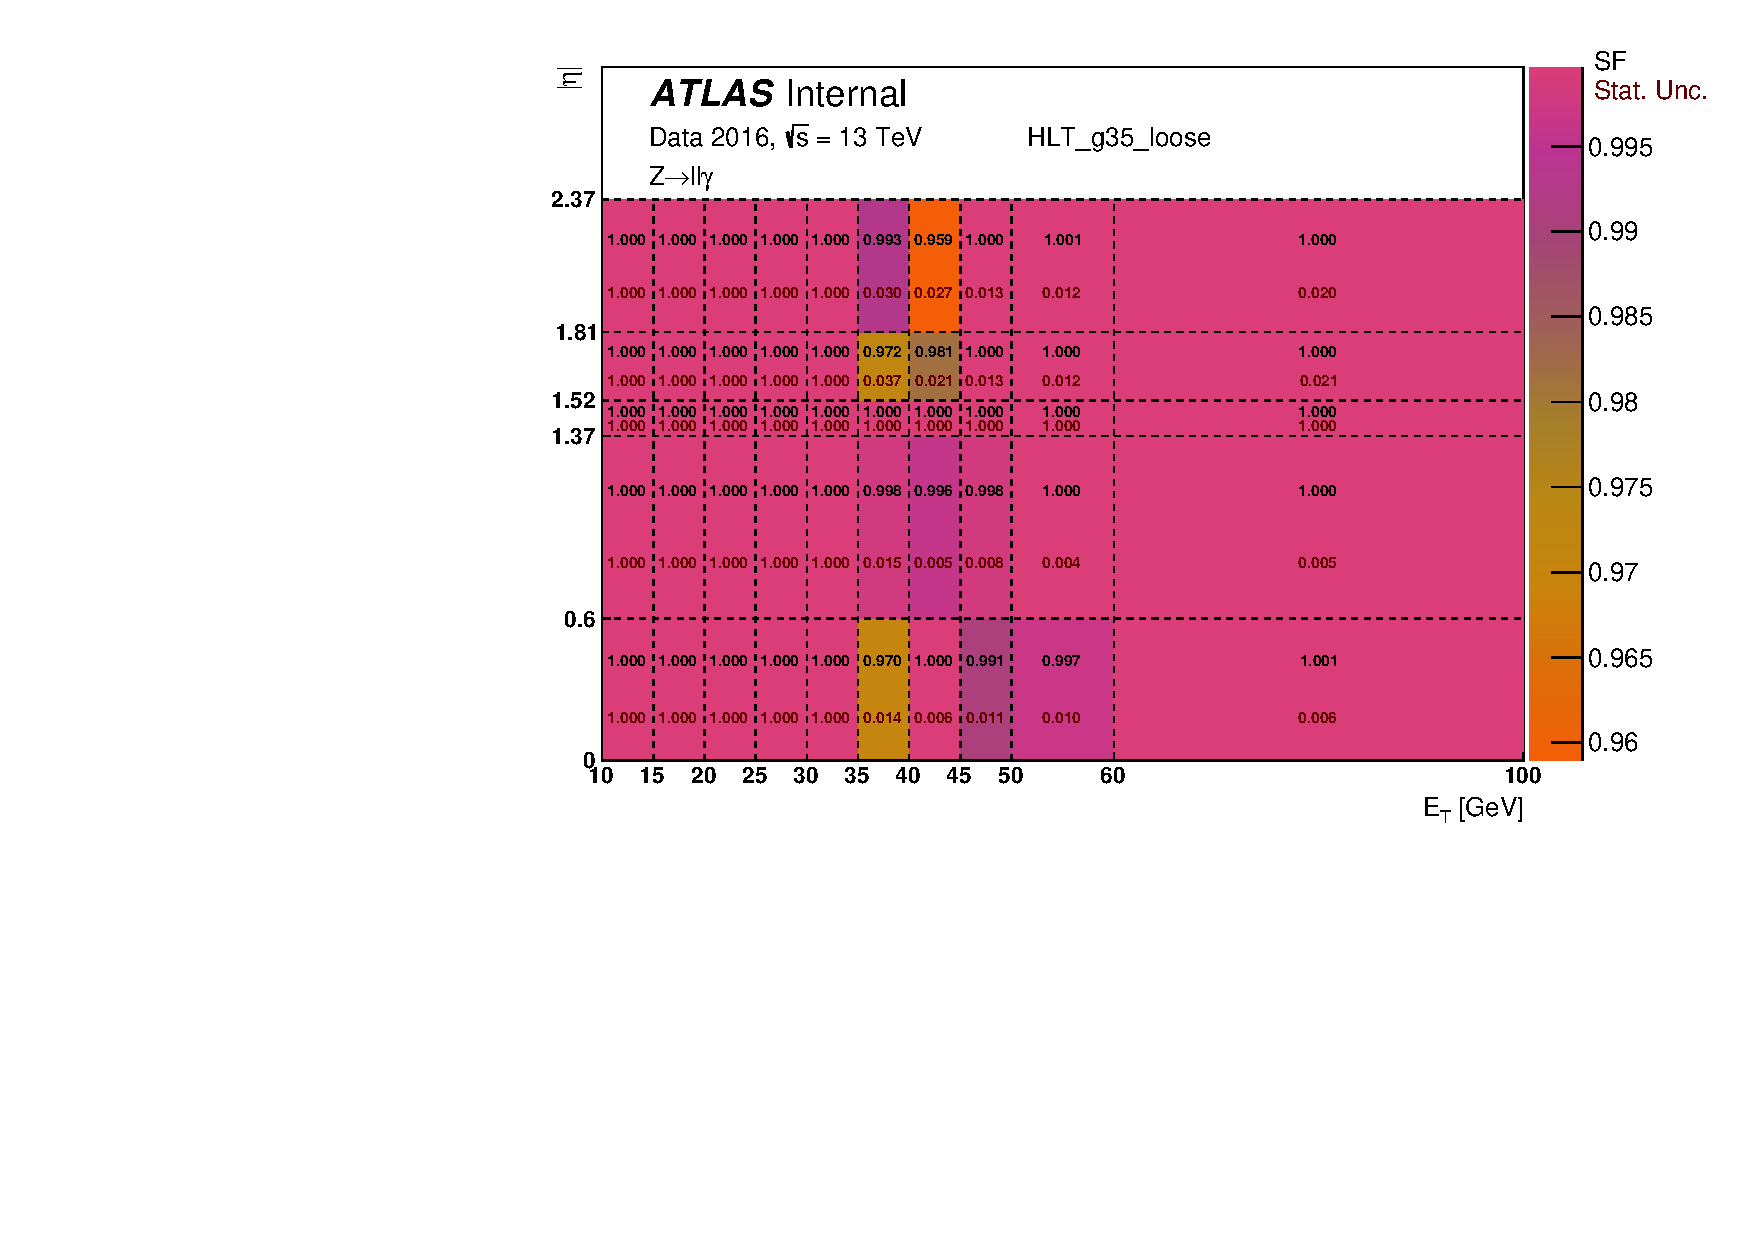
\includegraphics[width=0.45\textwidth]{images/trigger/2016_h_sf_et_eta_tr_HLT_g35_loose_FixedCutTightCaloOnly.pdf}}
      \caption{Scale Factors para el trigger \texttt{HLT\_g35\_loose} en función de $\ET$ y $\eta$ con un WP de aislamiento \texttt{FixedCutTightCaloOnly}, para el año 2015 (izquierda) y 2016 (derecha). En rojo las incertezas estadísticas.}
      \label{fig:SFs_2015_2016}
\end{figure}
\begin{figure}[!htpb]
  \centering
      {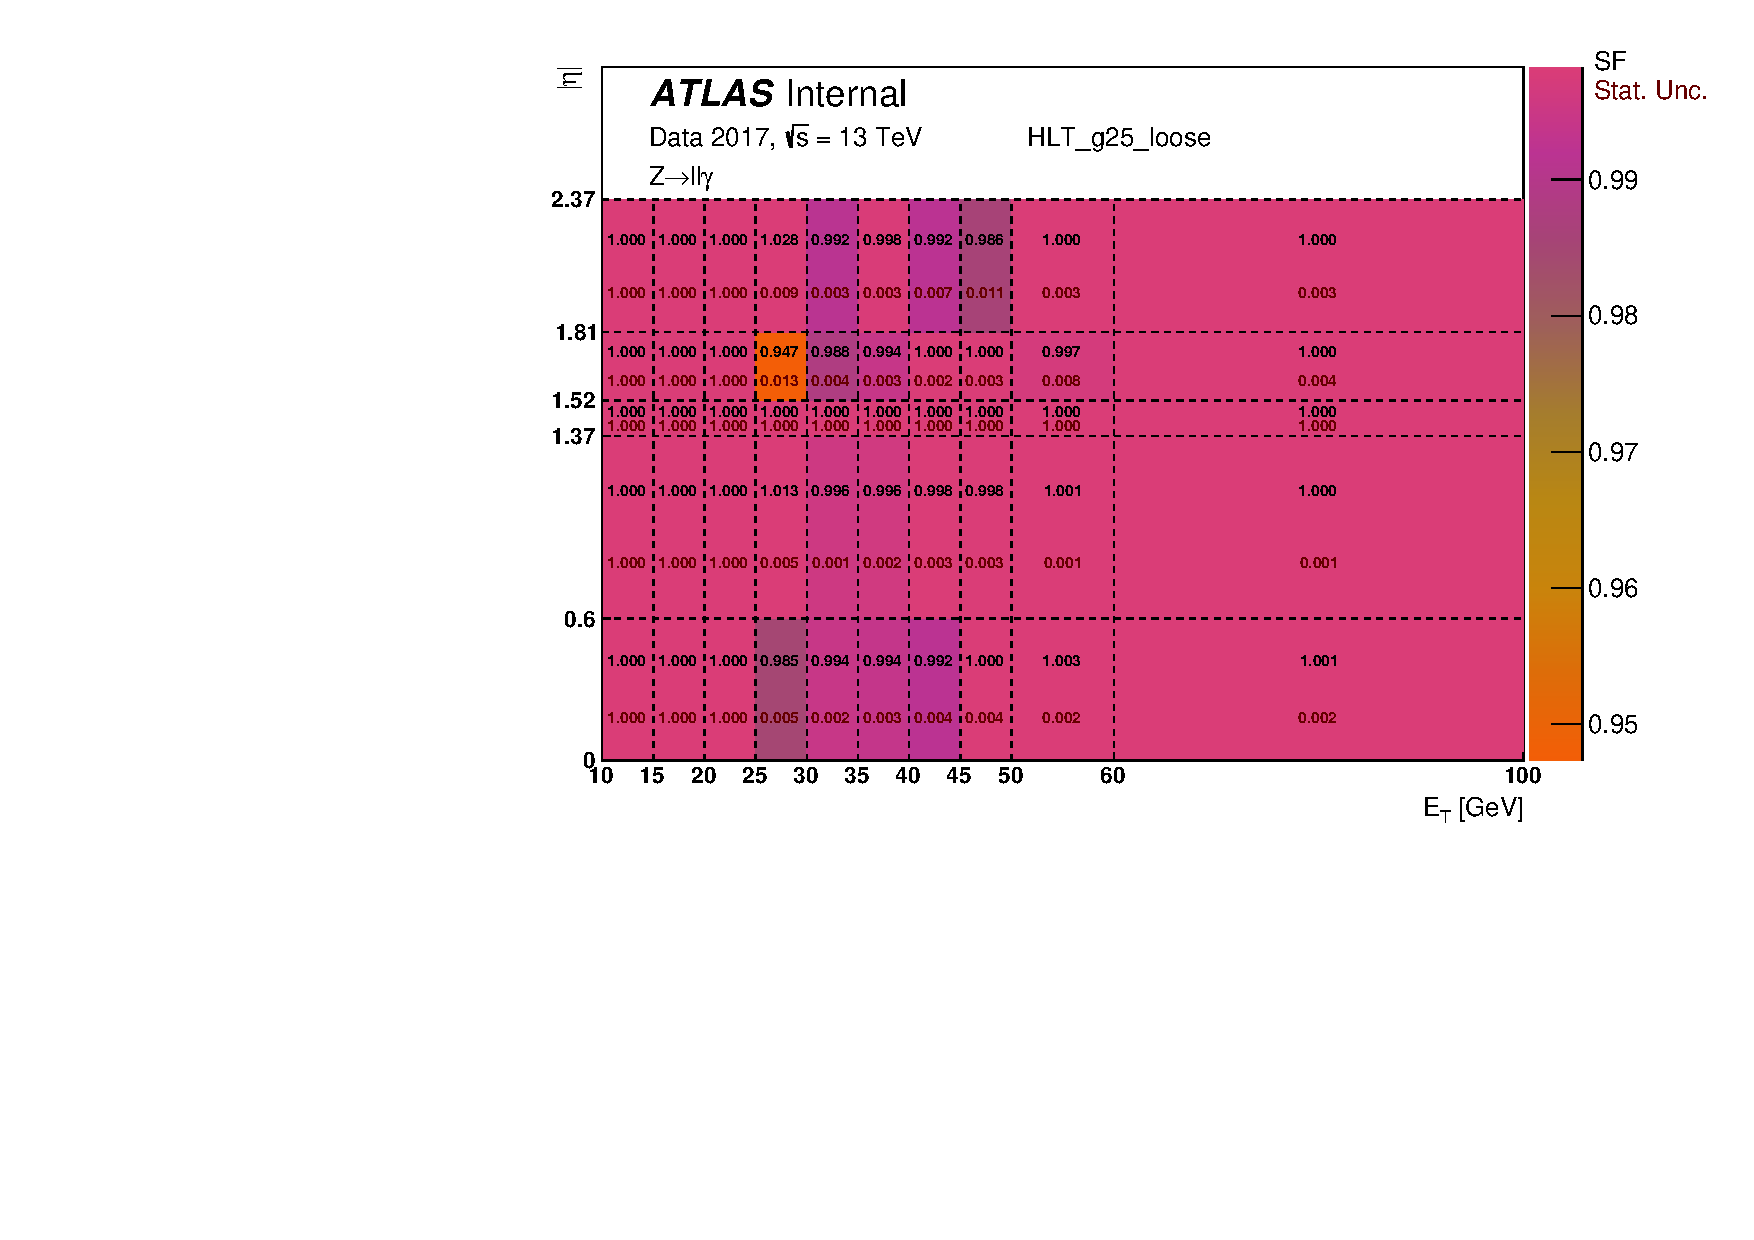
\includegraphics[width=0.45\textwidth]{images/trigger/2017_h_sf_et_eta_tr_HLT_g25_loose_FixedCutTightCaloOnly.pdf}}
      {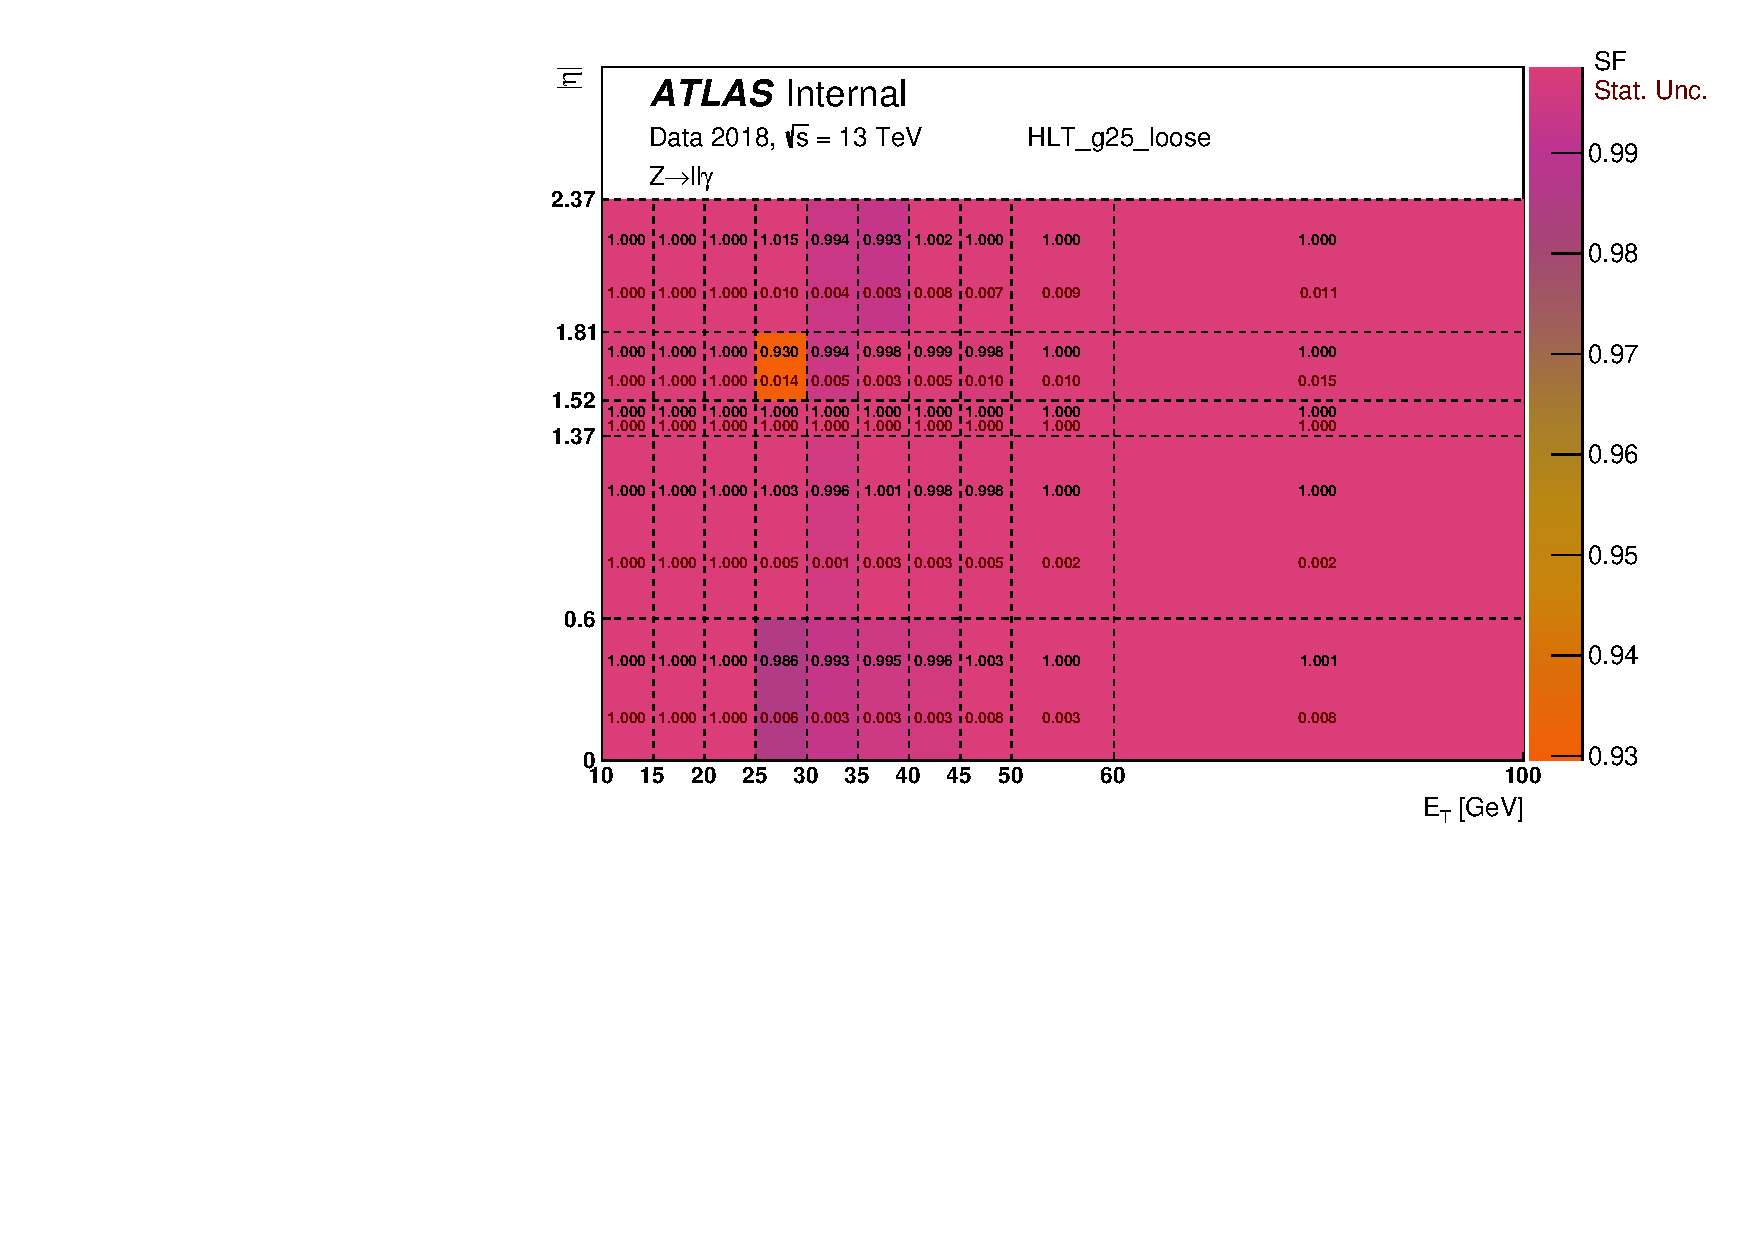
\includegraphics[width=0.45\textwidth]{images/trigger/2018_h_sf_et_eta_tr_HLT_g25_loose_FixedCutTightCaloOnly.pdf}}
      \caption{Scale Factors para el trigger \texttt{HLT\_g25\_loose} en función de $\ET$ y $\eta$ con un WP de aislamiento \texttt{FixedCutTightCaloOnly}, para el año 2017 (izquierda) y 2018 (derecha). En rojo las incertezas estadísticas.}
      \label{fig:SFs_2017_2018}
\end{figure}


